\section{Evaluation}

In diesem Kapitel werden die erhobenen Profiling-Daten visualisiert und
ausgewertet. Abschließend erfolgt ein direkter Vergleich hinsichtlich der
maximalen Regelungsfrequenz und der Ausführungsdauer von Regelungsfunktionen.

Die Profiling-Daten werden mit einem Python-Skript verarbeitet und als
Gantt-Diagramm dargestellt (\ref{fig:micro_ros_profiling},
\ref{fig:freertos_profiling}).

\begin{figure}[H]
    \centering
    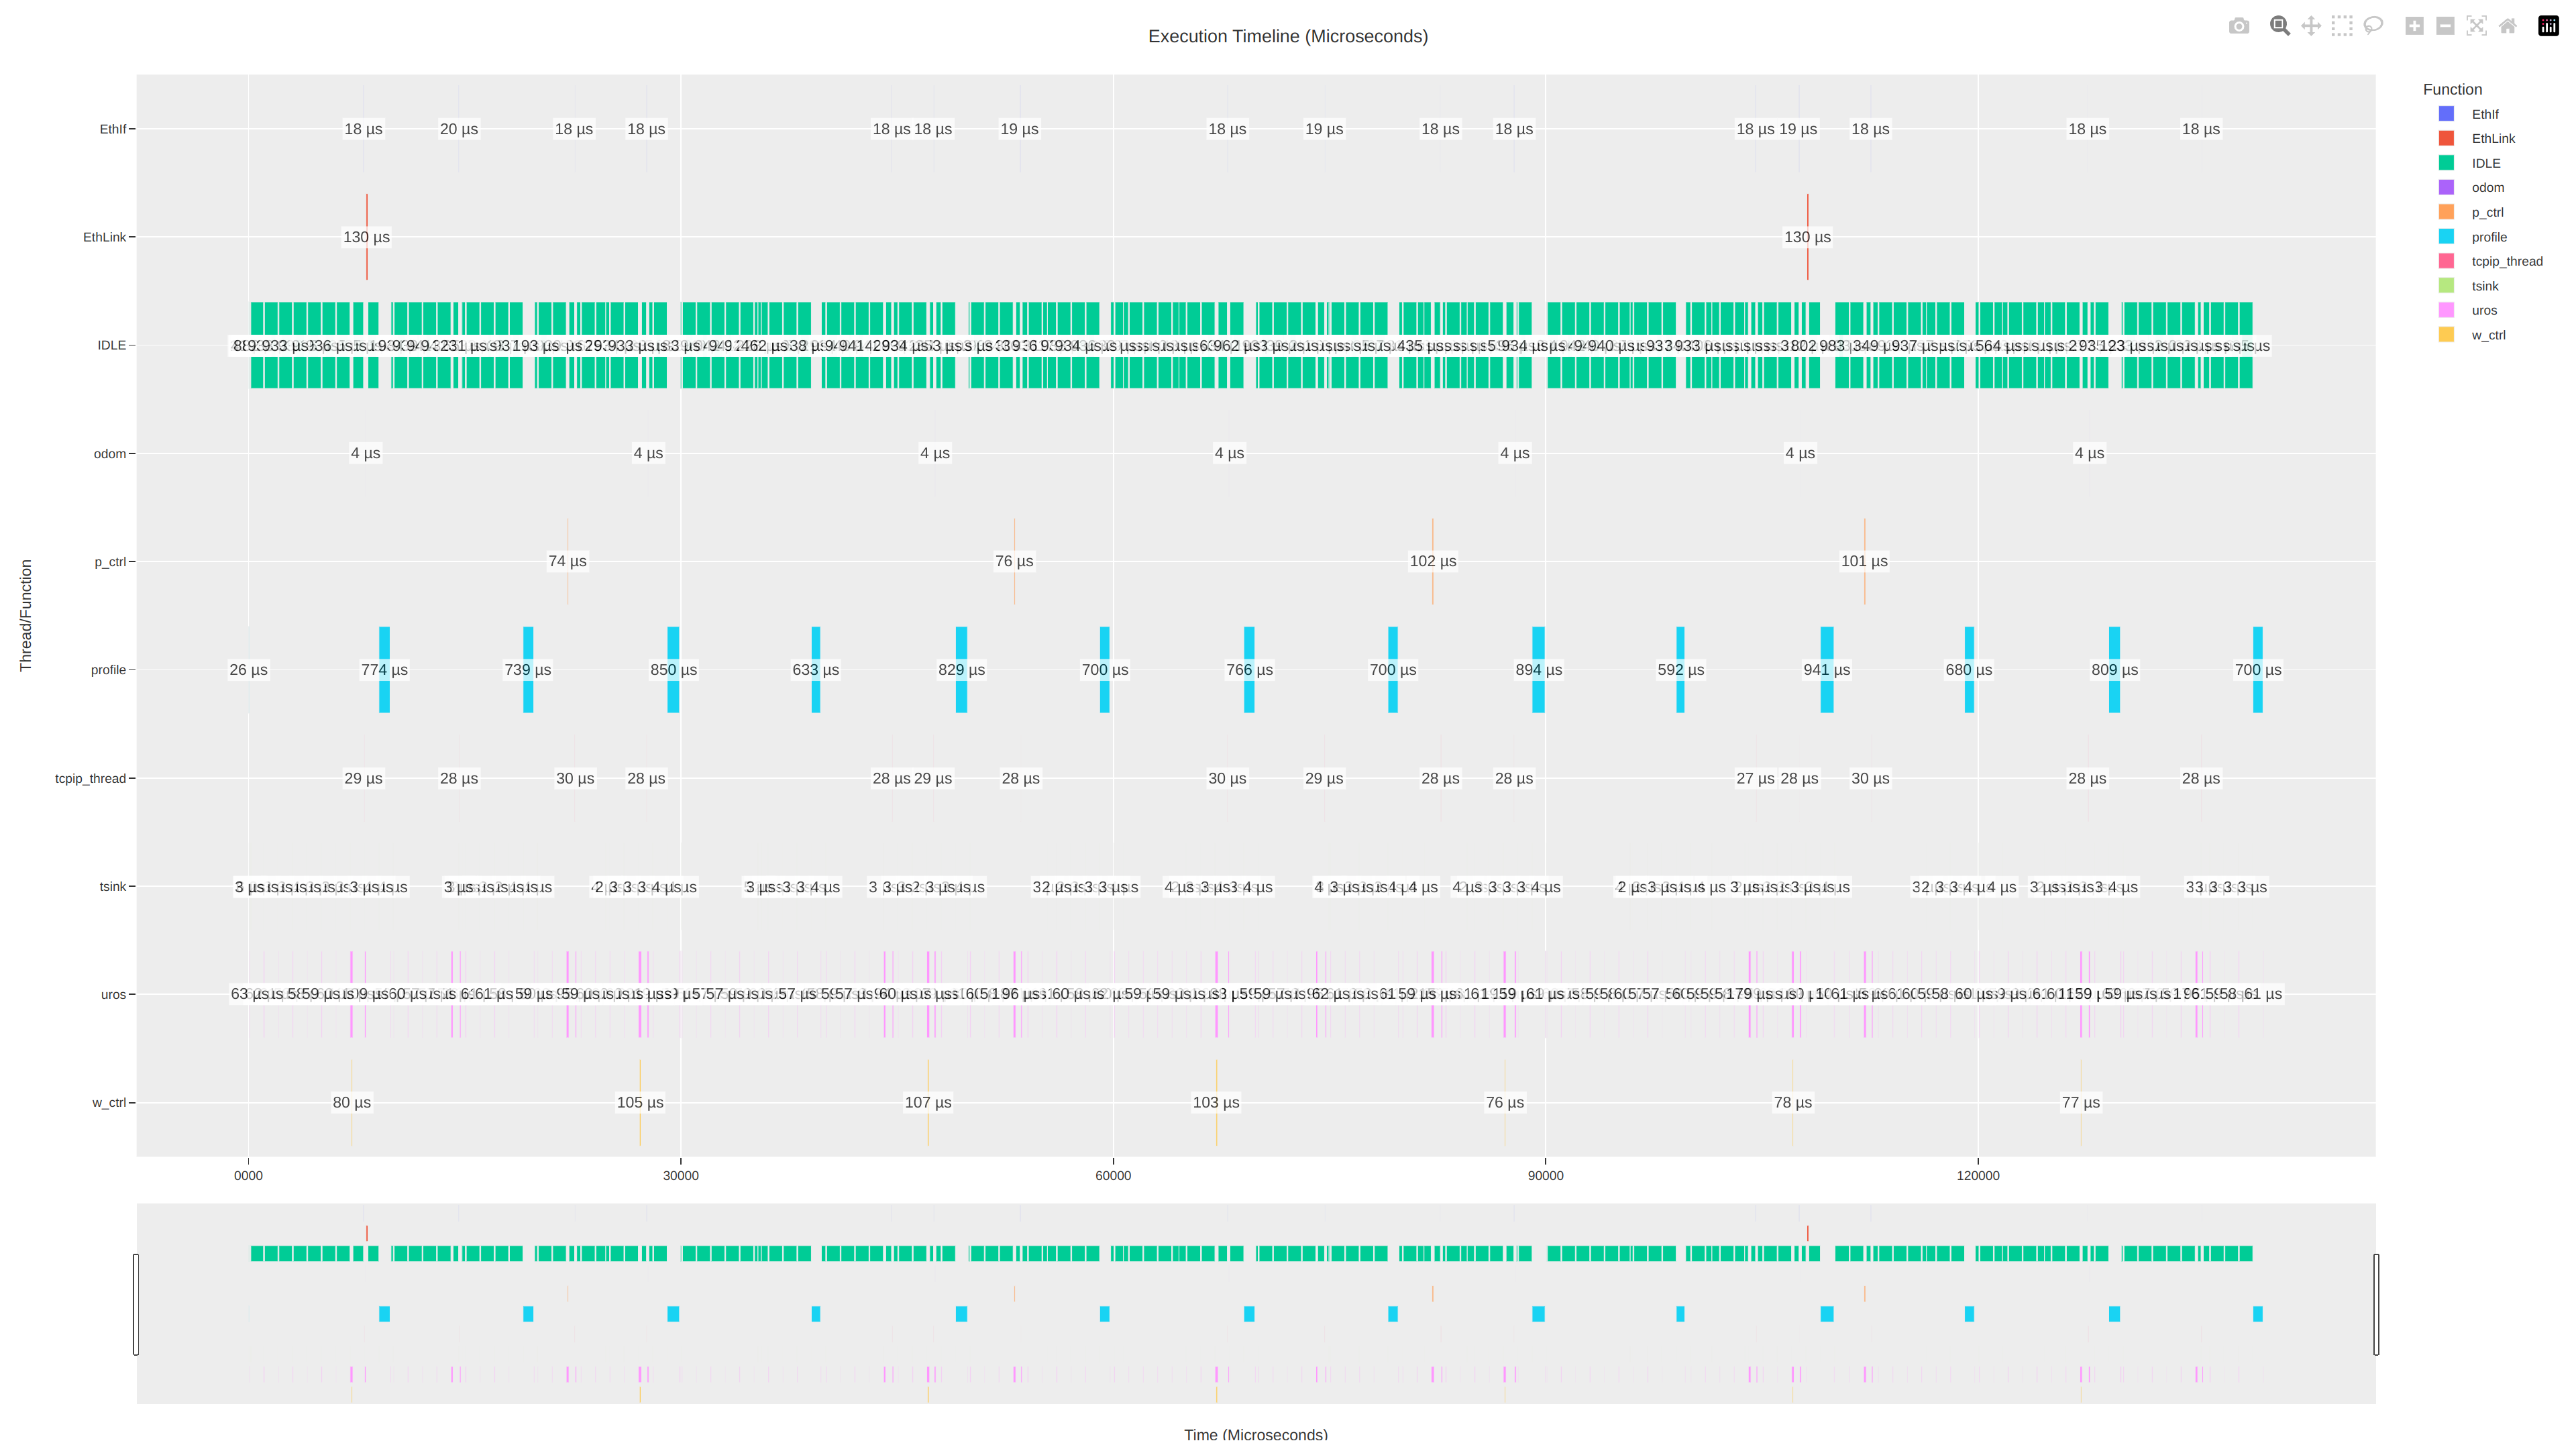
\includegraphics[width=0.95\textwidth]{assets/micro_ros_profiling}
    \caption{Laufzeit-Statistik unter Micro-ROS -- Überblick}
    \label{fig:micro_ros_profiling}
\end{figure}

\begin{figure}[H]
    \centering
    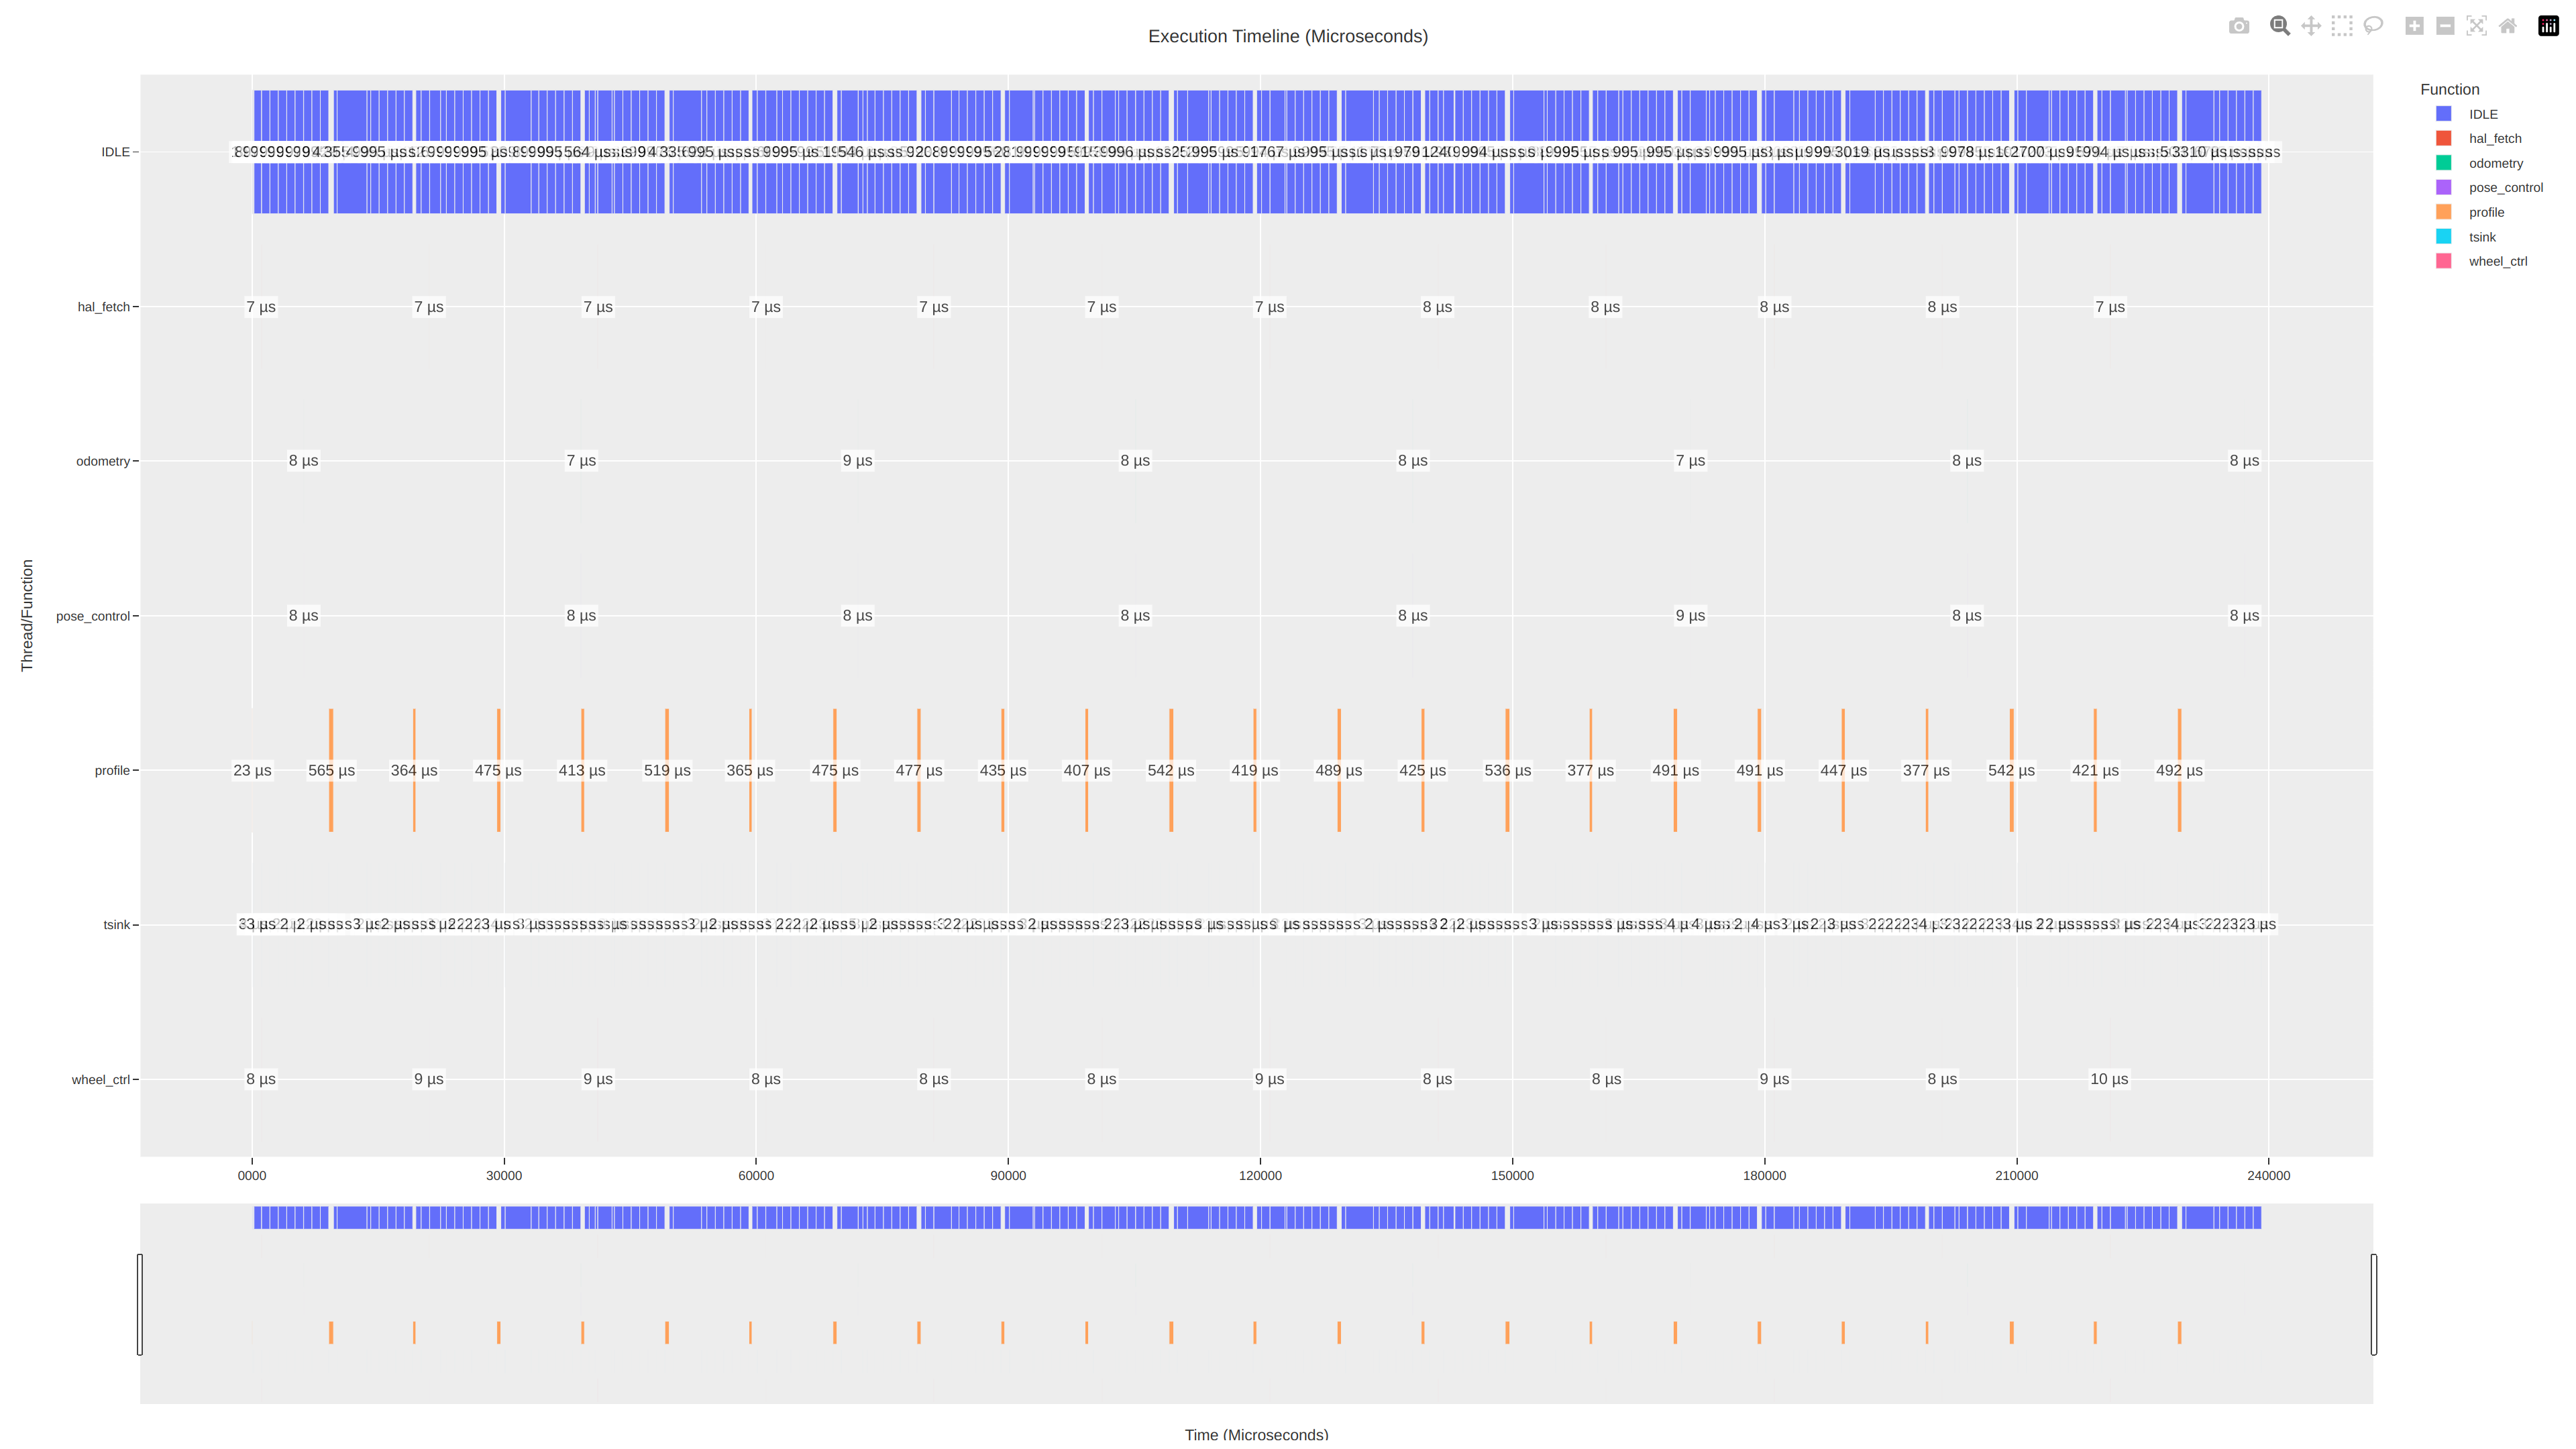
\includegraphics[width=0.95\textwidth]{assets/freertos_profiling}
    \caption{Laufzeit-Statistik unter FreeRTOS -- Überblick}
    \label{fig:freertos_profiling}
\end{figure}

Die FreeRTOS-Funktionen \mintinline{cpp}|vTaskGetRunTimeStats()| und
\mintinline{cpp}|vTaskList()| werden genutzt, um am Ende eines Samplings eine
grob zusammenfassende Auswertung bereitzustellen
(\ref{code:freertos_summary_uros}, \ref{code:freertos_summary_freertos}). Diese
dokumentieren die kumulierten Ausführungszeiten sowie Zustände aller Tasks vom
Systemstart bis zum Funktionsaufruf \cite{freertos_runtime_stats}.

\begin{minipage}[t]{0.5\textwidth}
\begin{code}
    \begin{minted}[linenos=false]{cpp}
=======================================
free heap:          4688
ctx switches:       126810
Task            Time        %
profile         33450       2%
uros            106984      8%
IDLE            1179311     88%
EthLink         1695        <1%
tcpip_thread    4526        <1%
tsink           3762        <1%
Tmr Svc         0           <1%
EthIf           2730        <1%
---------------------------------------
Task        State   Prio    Stack   Num
uros            R     24     2548     3
profile         X     24     892      2
IDLE            R     0      108      4
tcpip_thread    B     24     180      6
tsink           B     32     475      1
EthLink         B     16     193      8
EthIf           B     48     17       7
Tmr Svc         B     2      223      5
=======================================
profiled for 18881864 us
\end{minted}
    \captionof{listing}{Auswertung Micro-ROS}
    \label{code:freertos_summary_uros}
\end{code}
\end{minipage}
\hfill
\begin{minipage}[t]{0.5\textwidth}
\begin{code}
\begin{minted}[linenos=false]{cpp}
=======================================
free heap:          195696
ctx switches:       76148
Task            Time        %%
profile         9669        4%
IDLE            201086      95%
hal_fetch       81          <1%
wheel_ctrl      87          <1%
odometry        49          <1%
pose_control    51          <1%
tsink           615         <1%
Tmr Svc         0           <1%
recv_vel        0           <1%
---------------------------------------
Task        State   Prio    Stack   Num
profile         X      24     900     7
IDLE            R      0      108     8
wheel_ctrl      B      24     420     5
odometry        B      24     416     6
pose_control    B      24     410     4
tsink           B      32     483     1
hal_fetch       B      24     443     2
recv_vel        S      24     441     3
Tmr Svc         B      2      223     9
=======================================
profiled for 18779120 us
\end{minted}
    \captionof{listing}{Auswertung FreeRTOS}
    \label{code:freertos_summary_freertos}
\end{code}
\end{minipage}

Die Abbildung \ref{fig:profiling_ausschnitt} zeigt einen vergrößerten
Ausschnitt, der die Kontextwechsel visualisiert. Die gesamte Steuerungslogik
wird ausschließlich innerhalb der Micro-ROS-Task (\mintinline{text}|uros| in
Pink) verarbeitet, weswegen nur sie alle Regelungsfunktionen zeitlich überdeckt.

\begin{figure}[H]
    \centering
    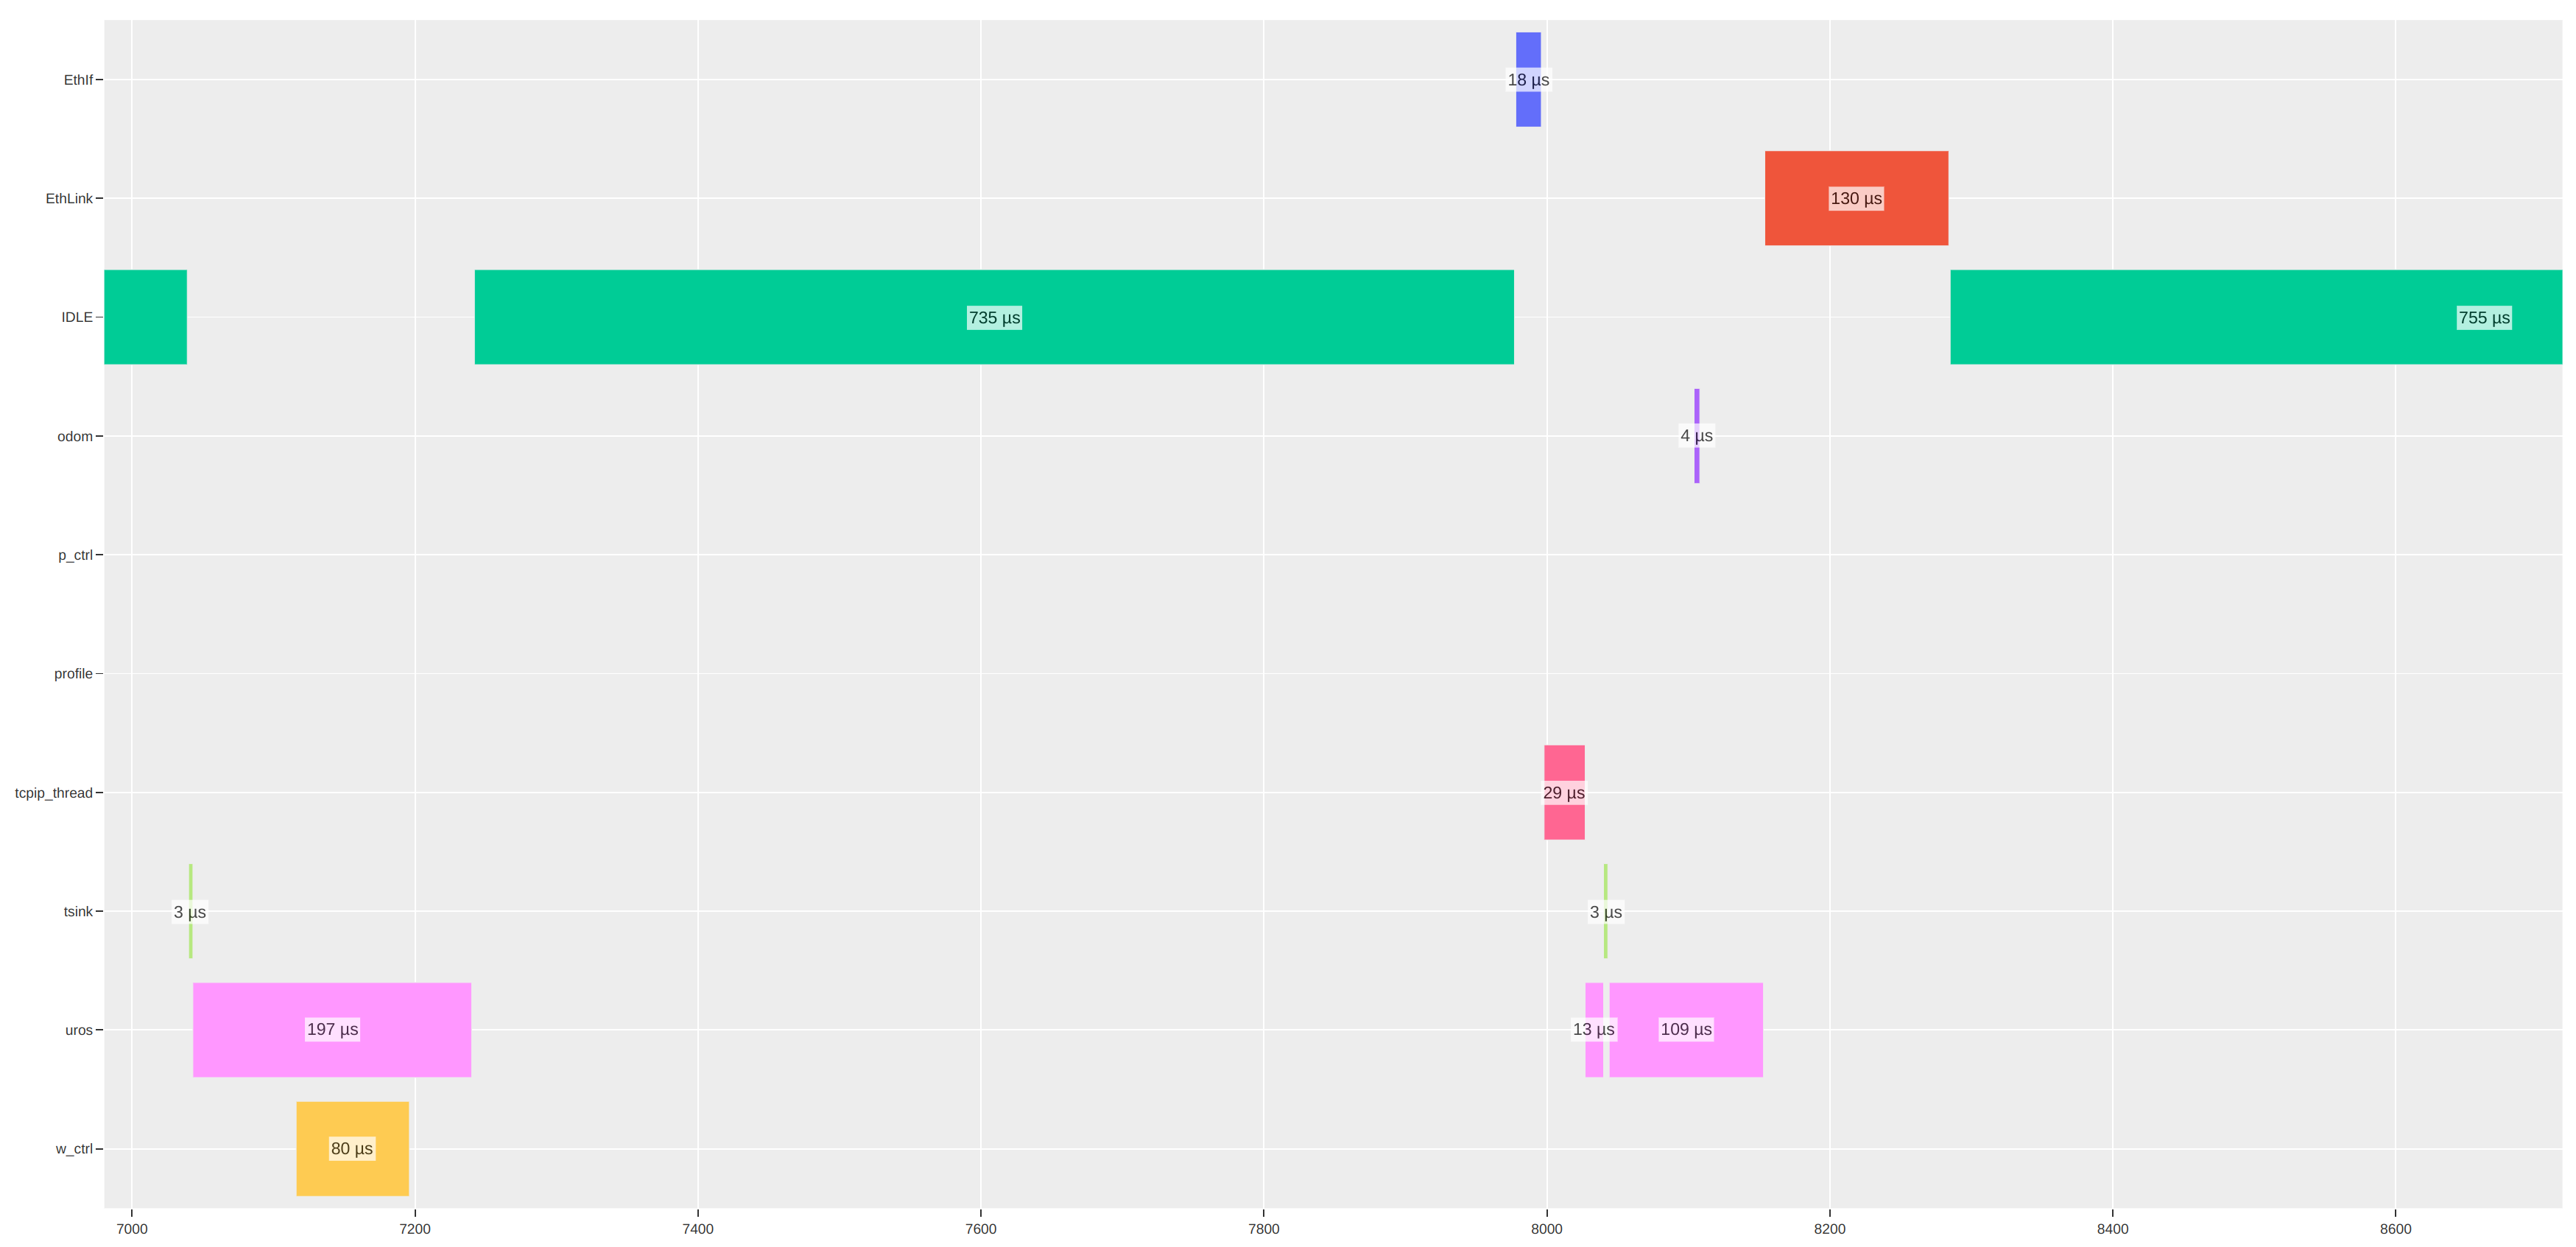
\includegraphics[width=1\textwidth]{assets/micro_ros_profiling_ausschnitt_cache_enabled}
    \caption{Laufzeit-Statistik unter Micro-ROS -- Ausschnitt}
    \label{fig:profiling_ausschnitt}
\end{figure}

\subsection{Laufzeit-Statistik -- Micro-ROS}

Die Profiling-Daten werden nun pro Task/Funktion separat aufsummiert und der
jeweilige Durchschnittswert berechnet.

Bei einer Sollfrequenz von $50\,\text{Hz}$ für die Drehzahlregelung und
$30\,\text{Hz}$ für die Posenregelung sowie Odometrie zeigen die Messergebnisse
nach etwa $18$ Sekunden Sampling folgende Werte -- jeweils ohne und mit Nutzung
von Caches:

\begin{table}[H]
\centering
\small
\setlength{\tabcolsep}{4pt}
\makebox[0pt][c]{\parbox{1.05\textwidth} \\ \hline
        \mintinline{text}|EthIf| & 52,93 & 115.022 & 0,62\,\% \\ \hline
        \mintinline{text}|EthLink| & 128,38 & 26.702 & 0,14\,\% \\ \hline
        \mintinline{text}|IDLE| & 587,79 & 8.961.378 & \textbf{48,17\,\%} \\ \hline
        \mintinline{text}|odom| & 8,88 & 8.186 & \textbf{0,04\,\%} \\ \hline
        \mintinline{text}|p_ctrl| & 277,97 & 170.671 & \textbf{0,92\,\%} \\ \hline
        \mintinline{text}|profile| & 623,40 & 4.981.587 & \textbf{26,78\,\%} \\ \hline
        \mintinline{text}|tcpip_thread| & 71,16 & 176.607 & 0,95\,\% \\ \hline
        \mintinline{text}|tsink| & 8,80 & 120.659 & 0,65\,\% \\ \hline
        \mintinline{text}|uros| & 203,31 & 3.807.442 & \textbf{20,47\,\%} \\ \hline
        \mintinline{text}|w_ctrl| & 256,11 & 236.136 & \textbf{1,27\,\%} \\ \hline
        \hline
        \textbf{Summe} & - & 18.604.390 & 100,00\,\% \\ \hline
        \end{tabular}
        \caption{Laufzeit-Statistik ohne Caching}
    \end{minipage}
    \hfill
    \begin{minipage}[b]{0.50\hsize}\centering
        \begin{tabular}{|l|r|r|r|}
        \hline
        \textbf{Name}  & \textbf{Ø (µs)} & \textbf{Summe} & \textbf{\%} \\ \hline
        \mintinline{text}|EthIf| & 18,43 & 40.671 & 0,21\,\% \\ \hline
        \mintinline{text}|EthLink| & 123,53 & 24.583 & 0,13\,\% \\ \hline
        \mintinline{text}|IDLE| & 661,14 & 15.505.748 & \textbf{81,81\,\%} \\ \hline
        \mintinline{text}|odom| & 4,02 & 3.791 & \textbf{0,02\,\%} \\ \hline
        \mintinline{text}|p_ctrl| & 88,25 & 55.511 & \textbf{0,29\,\%} \\ \hline
        \mintinline{text}|profile| & 803,55 & 1.517.905 & \textbf{8,01\,\%} \\ \hline
        \mintinline{text}|tcpip_thread| & 28,29 & 63.613 & 0,34\,\% \\ \hline
        \mintinline{text}|tsink| & 3,37 & 41.113 & 0,22\,\% \\ \hline
        \mintinline{text}|uros| & 76,17 & 1.614.854 & \textbf{8,52\,\%} \\ \hline
        \mintinline{text}|w_ctrl| & 90,82 & 85.646 & \textbf{0,45\,\%} \\ \hline
        \hline
        \textbf{Summe} & - & 18.953.435 & 100,00\,\% \\ \hline
        \end{tabular}
        \caption{Laufzeit-Statistik mit Caching}
    \end{minipage}
}}
\end{table}

Bei einer $100\,\text{Hz}\text{|}50\,\text{Hz}$-Reglerkonfiguration zeigen die
Messergebnisse nach etwa $18$ Sekunden Sampling folgende Werte -- jeweils ohne
und mit Nutzung von Caches:

\begin{table}[H]
\centering
\small
\setlength{\tabcolsep}{4pt}
\makebox[0pt][c]{\parbox{1.05\textwidth} \\ \hline
        \mintinline{text}|EthIf| & 51,53 & 198.643 & 1,05\,\% \\ \hline
        \mintinline{text}|EthLink| & 110,25 & 26.130 & 0,14\,\% \\ \hline
        \mintinline{text}|IDLE| & 545,36 & 7.330.732 & \textbf{38,75\,\%} \\ \hline
        \mintinline{text}|odom| & 9,92 & 18.149 & \textbf{0,10\,\%} \\ \hline
        \mintinline{text}|p_ctrl| & 322,41 & 295.008 & \textbf{1,56\,\%} \\ \hline
        \mintinline{text}|profile| & 566,25 & 5.472.282 & \textbf{28,92\,\%} \\ \hline
        \mintinline{text}|tcpip_thread| & 71,13 & 296.128 & 1,57\,\% \\ \hline
        \mintinline{text}|tsink| & 8,80 & 113.096 & 0,60\,\% \\ \hline
        \mintinline{text}|uros| & 231,74 & 4.606.256 & \textbf{24,35\,\%} \\ \hline
        \mintinline{text}|w_ctrl| & 307,53 & 562.785 & \textbf{2,97\,\%} \\ \hline
        \hline
        \textbf{Summe} & -- & 18.919.209 & 100,00\,\% \\ \hline
        \end{tabular}
        \caption{Laufzeit-Statistik ohne Caching}
    \end{minipage}
    \hfill
    \begin{minipage}[b]{0.50\hsize}\centering
        \begin{tabular}{|l|r|r|r|}
        \hline
        \textbf{Name}  & \textbf{Ø (µs)} & \textbf{Summe} & \textbf{\%} \\ \hline
        \mintinline{text}|EthIf| & 18,81 & 68.712 & 0,37\,\% \\ \hline
        \mintinline{text}|EthLink| & 128,88 & 23.971 & 0,13\,\% \\ \hline
        \mintinline{text}|IDLE| & 607,96 & 14.540.662 & \textbf{78,00\,\%} \\ \hline
        \mintinline{text}|odom| & 3,74 & 6.780 & \textbf{0,04\,\%} \\ \hline
        \mintinline{text}|p_ctrl| & 75,16 & 69.301 & \textbf{0,37\,\%} \\ \hline
        \mintinline{text}|profile| & 889,48 & 1.641.972 & \textbf{8,81\,\%} \\ \hline
        \mintinline{text}|tcpip_thread| & 28,25 & 104.623 & 0,56\,\% \\ \hline
        \mintinline{text}|tsink| & 3,43 & 36.583 & 0,20\,\% \\ \hline
        \mintinline{text}|uros| & 86,44 & 1.957.616 & \textbf{10,50\,\%} \\ \hline
        \mintinline{text}|w_ctrl| & 103,59 & 191.027 & \textbf{1,02\,\%} \\ \hline
        \hline
        \textbf{Summe} & -- & 18.641.247 & 100,00\,\% \\ \hline
        \end{tabular}
        \caption{Laufzeit-Statistik mit Caching}
    \end{minipage}
}}
\end{table}

Ohne Daten- oder Instruktionscache benötigte die Micro-ROS-Task für unter
anderem die gesamte Steuerungslogik bei den Reglern mit $50\,\text{Hz}$ sowie
$30\,\text{Hz}$ $\textbf{20,47\,\%}$ Rechenzeit. Bei $100\,\text{Hz}$ sowie
$50\,\text{Hz}$ waren es $\textbf{24,35\,\%}$. Gleichzeitig befand sich das
System zu $\textbf{48,17\,\%}$ bzw. $\textbf{38,75\,\%}$ im Leerlauf.

Mit aktiviertem Daten- und Instruktionscache benötigte die Micro-ROS-Task bei
den Reglern mit $50\,\text{Hz}$ sowie $30\,\text{Hz}$ nur $\textbf{8,52\,\%}$
Rechenzeit. Bei höheren Frequenzen ($100\,\text{Hz}$ sowie $50\,\text{Hz}$) ist
sie $\textbf{10,50\,\%}$, während die Leerlaufzeit bei $\textbf{81,81\,\%}$ bzw.
$\textbf{78,00\,\%}$ liegt.

Durch die Nutzung der Caches reduzierte sich die Rechenzeit für die Roboterlogik
beispielsweise in der $100\,\text{Hz}/50\,\text{Hz}$-Reglerkonfiguration
deutlich: um $\textbf{62,64\,\%}$ für die Odometrie, $\textbf{76,51\,\%}$ für
die Posenregelung und $\textbf{66,06\,\%}$ für die Drehzahlregelung.
Gleichzeitig stieg die Leerlaufzeit um $\textbf{98,35\,\%}$ an, wobei die
gesamte Profiling-Dauer zwischen den beiden Samplings eine Differenz von
$349,\!045\,\text{ms}$ aufwies.

\subsection{Laufzeit-Statistik -- FreeRTOS}

Bei einer $50\,\text{Hz}\text{|}30\,\text{Hz}$-Reglerkonfiguration zeigen die
Messergebnisse nach etwa $18$ Sekunden Sampling folgende Werte -- jeweils ohne
und mit Nutzung von Caches:

\begin{table}[H]
\centering
\small
\setlength{\tabcolsep}{4pt}
\makebox[0pt][c]{\parbox{1.05\textwidth} \\ \hline
        \mintinline{text}|IDLE| & 983,50 & 14.996.422 & \textbf{81,85\%} \\ \hline
        \mintinline{text}|hal_fetch| & 21,71 & 20.403 & 0,11\% \\ \hline
        \mintinline{text}|odometry| & 24,05 & 13.634 & \textbf{0,07\%} \\ \hline
        \mintinline{text}|pose_control| & 32,66 & 18.682 & \textbf{0,10\%} \\ \hline
        \mintinline{text}|profile| & 902,87 & 3.077.879 & \textbf{16,80\%} \\ \hline
        \mintinline{text}|tsink| & 9,63 & 161.451 & 0,88\% \\ \hline
        \mintinline{text}|wheel_ctrl| & 35,80 & 34.260 & \textbf{0,19\%} \\ \hline
        \hline
        \textbf{Summe} & -- & 18.322.731 & 100,00\,\% \\ \hline
        \end{tabular}
        \caption{Laufzeit-Statistik ohne Caching}
    \end{minipage}
    \hfill
    \begin{minipage}[b]{0.50\hsize}\centering
        \begin{tabular}{|l|r|r|r|}
        \hline
        \textbf{Name}  & \textbf{Ø (µs)} & \textbf{Summe} & \textbf{\%} \\ \hline
        \mintinline{text}|IDLE| & 1.041,06 & 17.658.382 & \textbf{94,83\,\%} \\ \hline
        \mintinline{text}|hal_fetch| & 6,43 & 6.003 & 0,03\,\% \\ \hline
        \mintinline{text}|odometry| & 7,19 & 4.068 & \textbf{0,02\,\%} \\ \hline
        \mintinline{text}|pose_control| & 9,64 & 5.456 & \textbf{0,03\,\%} \\ \hline
        \mintinline{text}|profile| & 476,43 & 889.027 & \textbf{4,77\,\%} \\ \hline
        \mintinline{text}|tsink| & 2,95 & 46.947 & 0,25\,\% \\ \hline
        \mintinline{text}|wheel_ctrl| & 10,96 & 10.379 & \textbf{0,06\,\%} \\ \hline
        \hline
        \textbf{Summe} & -- & 18.620.262 & 100,00\,\% \\ \hline
        \end{tabular}
        \caption{Laufzeit-Statistik mit Caching}
    \end{minipage}
}}
\end{table}

Bei einer $100\,\text{Hz}\text{|}50\,\text{Hz}$-Reglerkonfiguration zeigen die
Messergebnisse nach etwa $18$ Sekunden Sampling folgende Werte -- jeweils ohne
und mit Nutzung von Caches:

\begin{table}[H]
\centering
\small
\setlength{\tabcolsep}{4pt}
\makebox[0pt][c]{\parbox{1.05\textwidth} \\ \hline
        \mintinline{text}|IDLE| & 997,02 & 14.706.086 & \textbf{80,67\,\%} \\ \hline
        \mintinline{text}|hal_fetch| & 21,91 & 40.471 & 0,22\,\% \\ \hline
        \mintinline{text}|odometry| & 24,01 & 22.373 & \textbf{0,12\,\%} \\ \hline
        \mintinline{text}|pose_control| & 32,46 & 30.579 & \textbf{0,17\,\%} \\ \hline
        \mintinline{text}|profile| & 941,93 & 3.209.167 & \textbf{17,60\,\%} \\ \hline
        \mintinline{text}|tsink| & 9,36 & 151.046 & 0,83\,\% \\ \hline
        \mintinline{text}|wheel_ctrl| & 37,77 & 70.285 & \textbf{0,39\,\%} \\ \hline
        \hline
        \textbf{Summe} & {--} & 18.230.007 & 100,00\,\% \\ \hline
        \end{tabular}
        \caption{Laufzeit-Statistik ohne Caching}
    \end{minipage}
    \hfill
    \begin{minipage}[b]{0.50\hsize}\centering
        \begin{tabular}{|l|r|r|r|}
        \hline
        \textbf{Name}  & \textbf{Ø (µs)} & \textbf{Summe} & \textbf{\%} \\ \hline
        \mintinline{text}|IDLE| & 1.139,87 & 17.276.974 & \textbf{94,61\,\%} \\ \hline
        \mintinline{text}|hal_fetch| & 6,61 & 12.104 & 0,07\,\% \\ \hline
        \mintinline{text}|odometry| & 6,84 & 6.256 & \textbf{0,03\,\%} \\ \hline
        \mintinline{text}|pose_control| & 9,88 & 9.043 & \textbf{0,05\,\%} \\ \hline
        \mintinline{text}|profile| & 487,57 & 892.246 & \textbf{4,89\,\%} \\ \hline
        \mintinline{text}|tsink| & 3,01 & 45.597 & 0,25\,\% \\ \hline
        \mintinline{text}|wheel_ctrl| & 10,69 & 19.559 & \textbf{0,11\,\%} \\ \hline
        \hline
        \textbf{Summe} & {--} & 18.443.591 & 100.00\,\% \\ \hline
        \end{tabular}
        \caption{Laufzeit-Statistik mit Caching}
    \end{minipage}
}}
\end{table}

Ohne Micro-ROS-Abhängigkeit erreicht das System bereits ohne Caches eine
Leerlaufzeit von etwa $\textbf{80\,\%}$. Mit aktivierten Caches steigt diese auf
ungefähr $\textbf{95\,\%}$ an.

Die Leistungssteigerung durch die Nutzung von Caches ist bei der Implementierung
unter FreeRTOS ebenfalls signifikant, wobei sich die gesamte Profiling-Dauer
beider Samplings bei der $100\,\text{Hz}|50\,\text{Hz}$-Reglerkonfiguration um
$213,584\,\text{ms}$ unterscheidet: Die Rechenzeiten verringerten sich für die
Odometrie um $\textbf{72,04\,\%}$, für die Posenregelung um $\textbf{70,43\,\%}$
sowie für die Drehzahlregelung um $\textbf{72,17\,\%}$. Die Leerlaufzeit stieg
dabei um $\textbf{14,88\,\%}$, 

\subsection{Vergleich zwischen Micro-ROS und FreeRTOS}

\subsubsection{Experimentelle Bestimmung der maximalen Regelungsfrequenz}

Bei FreeRTOS gibt es keine theoretische Obergrenze für die Taktfrequenz zum
Kontextwechsel. Die praktische maximale Frequenz liegt standardmäßig bei
$1000\,\text{Hz}$, da der Tick-Interrupt (für den Kontextwechsel) standardmäßig
auf $1\,\text{ms}$ (entsprechend $1000$ Interrupts pro Sekunde) festgelegt ist.

Um eine Taktfrequenz für das FreeRTOS-System über $1000\,\text{Hz}$ zu
erreichen, muss lediglich der Wert des Makros
\mintinline{cpp}|configTICK_RATE_HZ| auf die gewünschte Frequenz angepasst
werden. Von Frequenzen über $1000\,\text{Hz}$ wird jedoch abgeraten, da die
kumulativen Kontextwechselkosten einen spürbaren Overhead verursachen
\cite{FreertosTickRate2010}. Bei hochfrequenten Systemen, die deutlich über die
Standardfrequenz für Kontextwechsel arbeiten, empfiehlt sich daher der Verzicht
auf ein RTOS zugunsten eines minimalen Schedulers \cite{FreertosForumHF2019}.

Wie in den Grafiken \ref{fig:freertos_1000hz} und
\ref{fig:freertos_1000hz_section} veranschaulicht, kann das Regelungssystem,
dessen zugrundeliegende Datenaustausch mittels FreeRTOS-APIs auf minimalen
Overhead optimiert wurde, problemlos mit $1000\,\text{Hz}$ betrieben werden. Die
Tasks werden rhythmisch und auch deterministisch jeweils mit den vorgegebenen
Frequenzen ausgeführt -- stets zum gleichen relativen Zeitpunkt zueinander.

\begin{figure}[H]
    \centering
    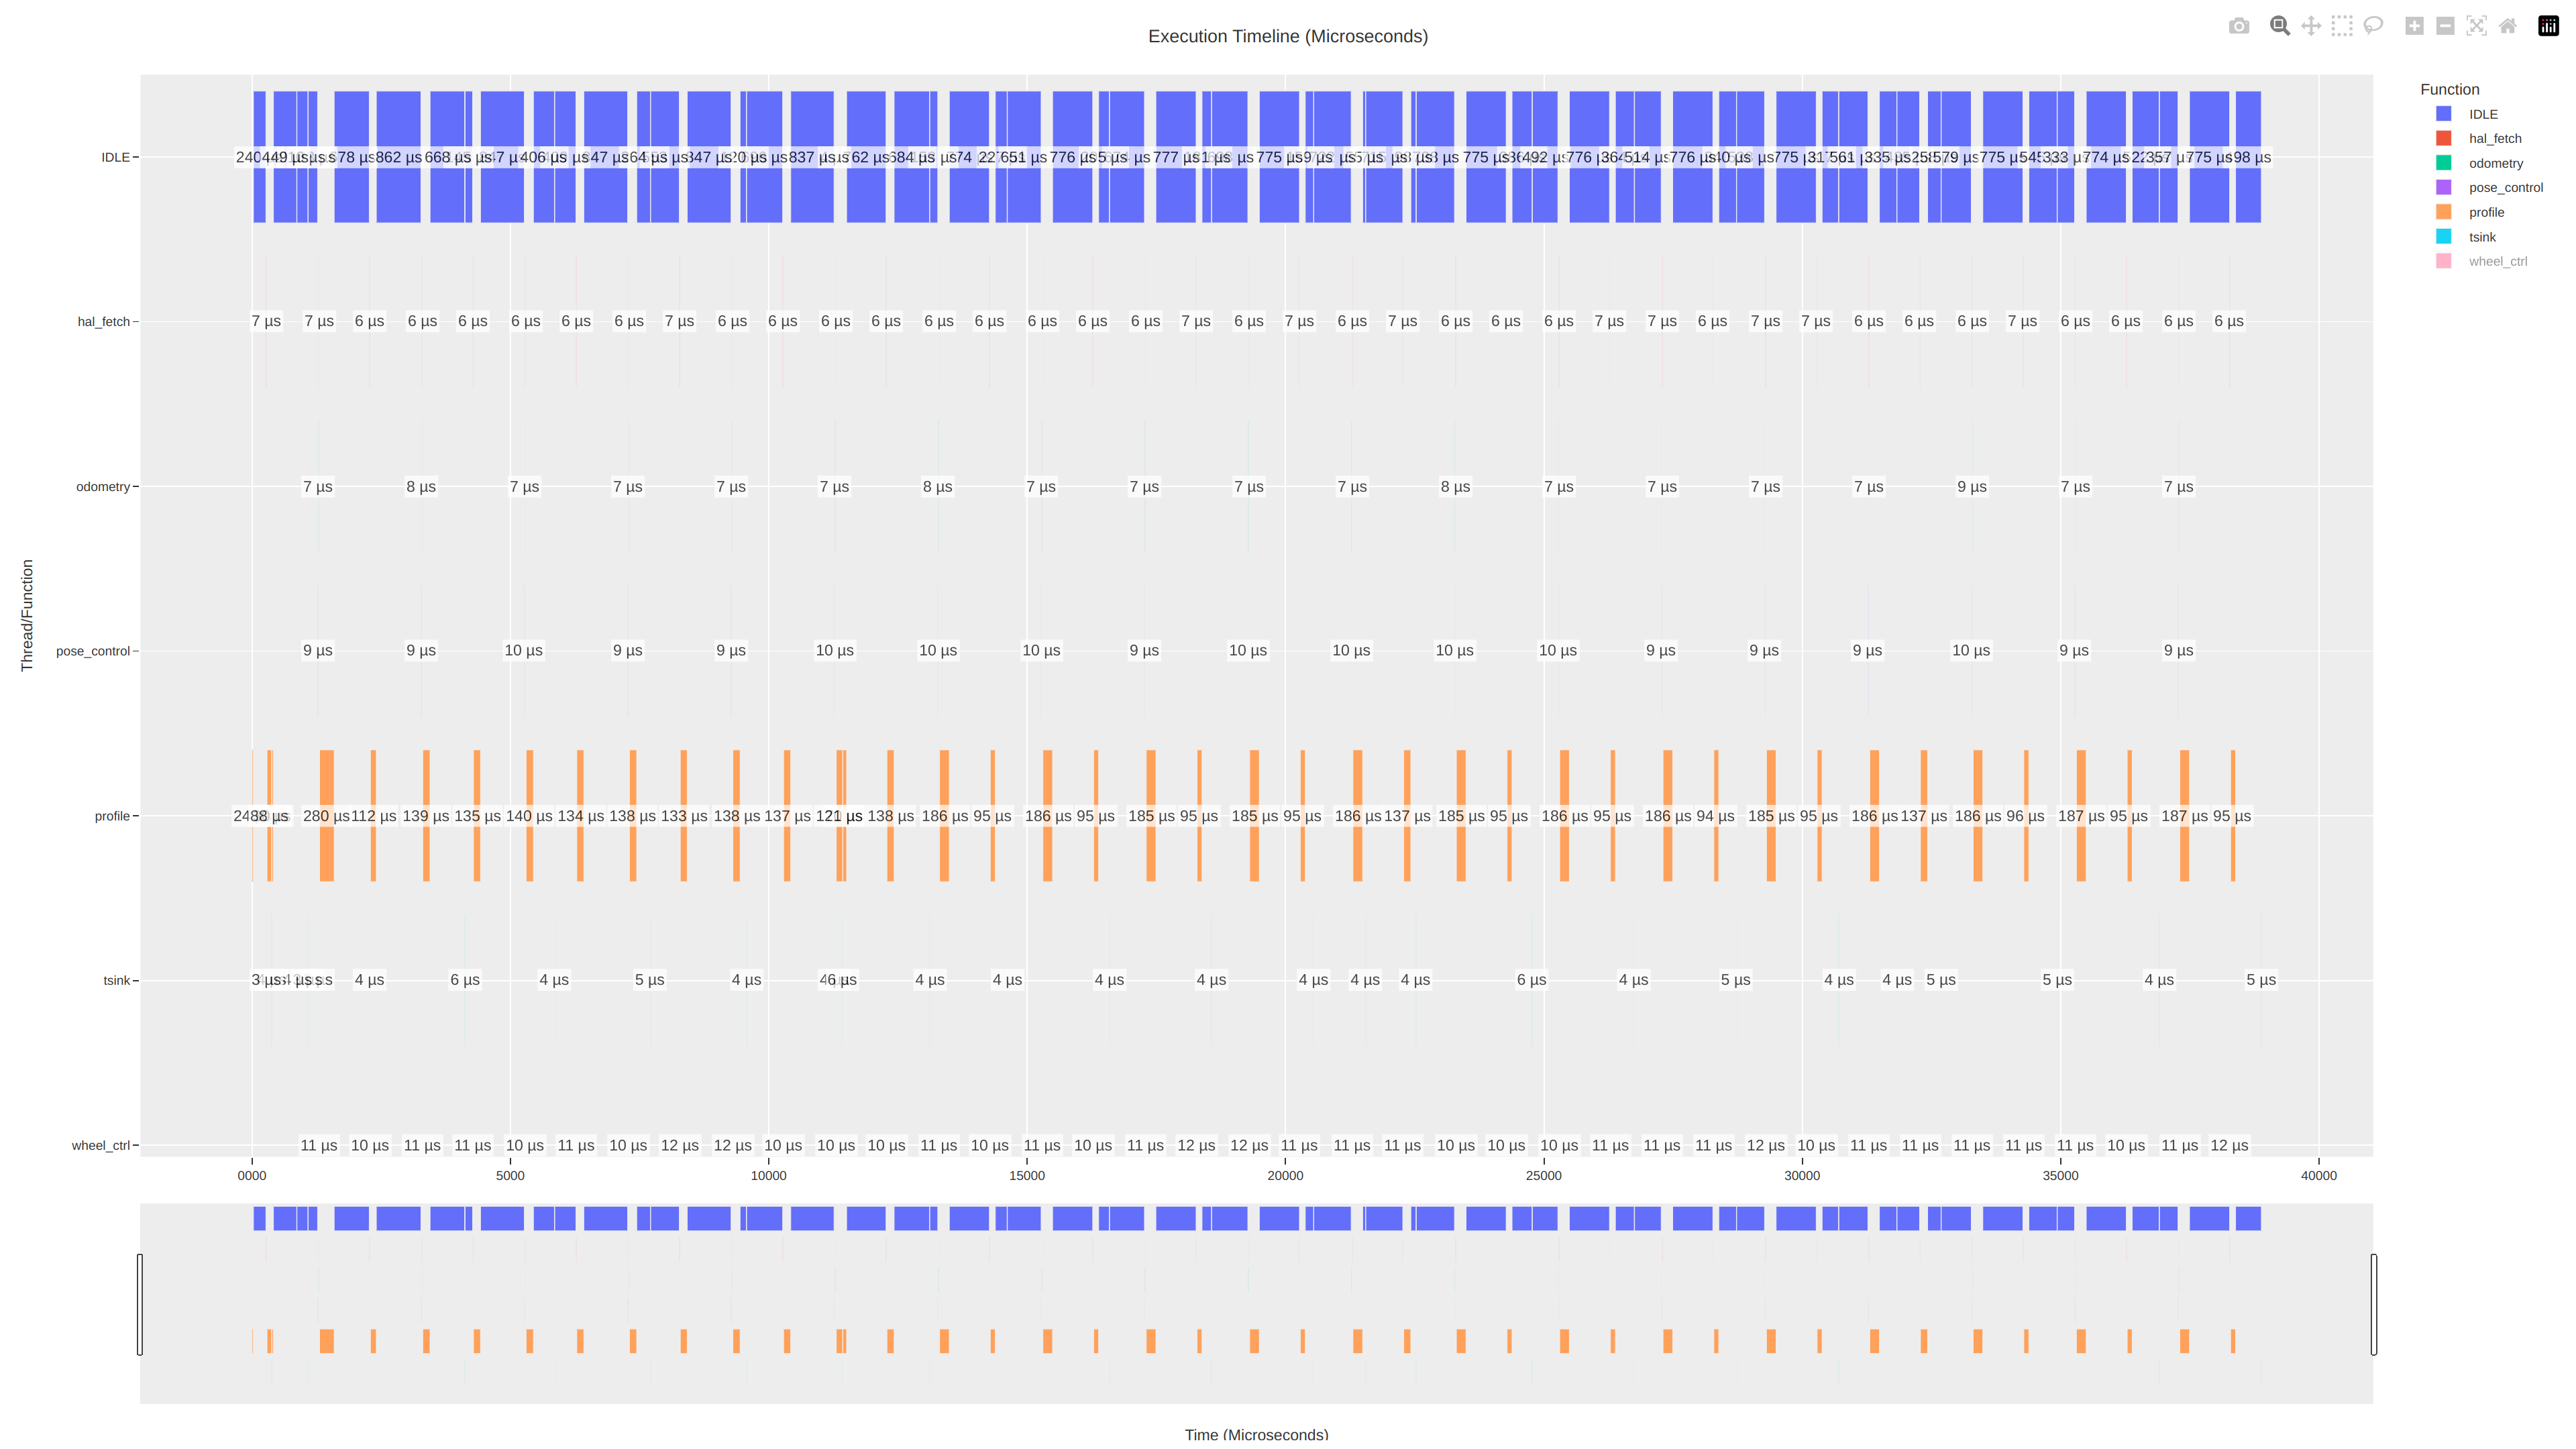
\includegraphics[width=1\textwidth]{assets/freertos_profiling_1000hz}
    \caption{Laufzeit-Statistik mit 1000 Hz unter FreeRTOS}
    \label{fig:freertos_1000hz}
\end{figure}
\begin{figure}[H]
    \centering
    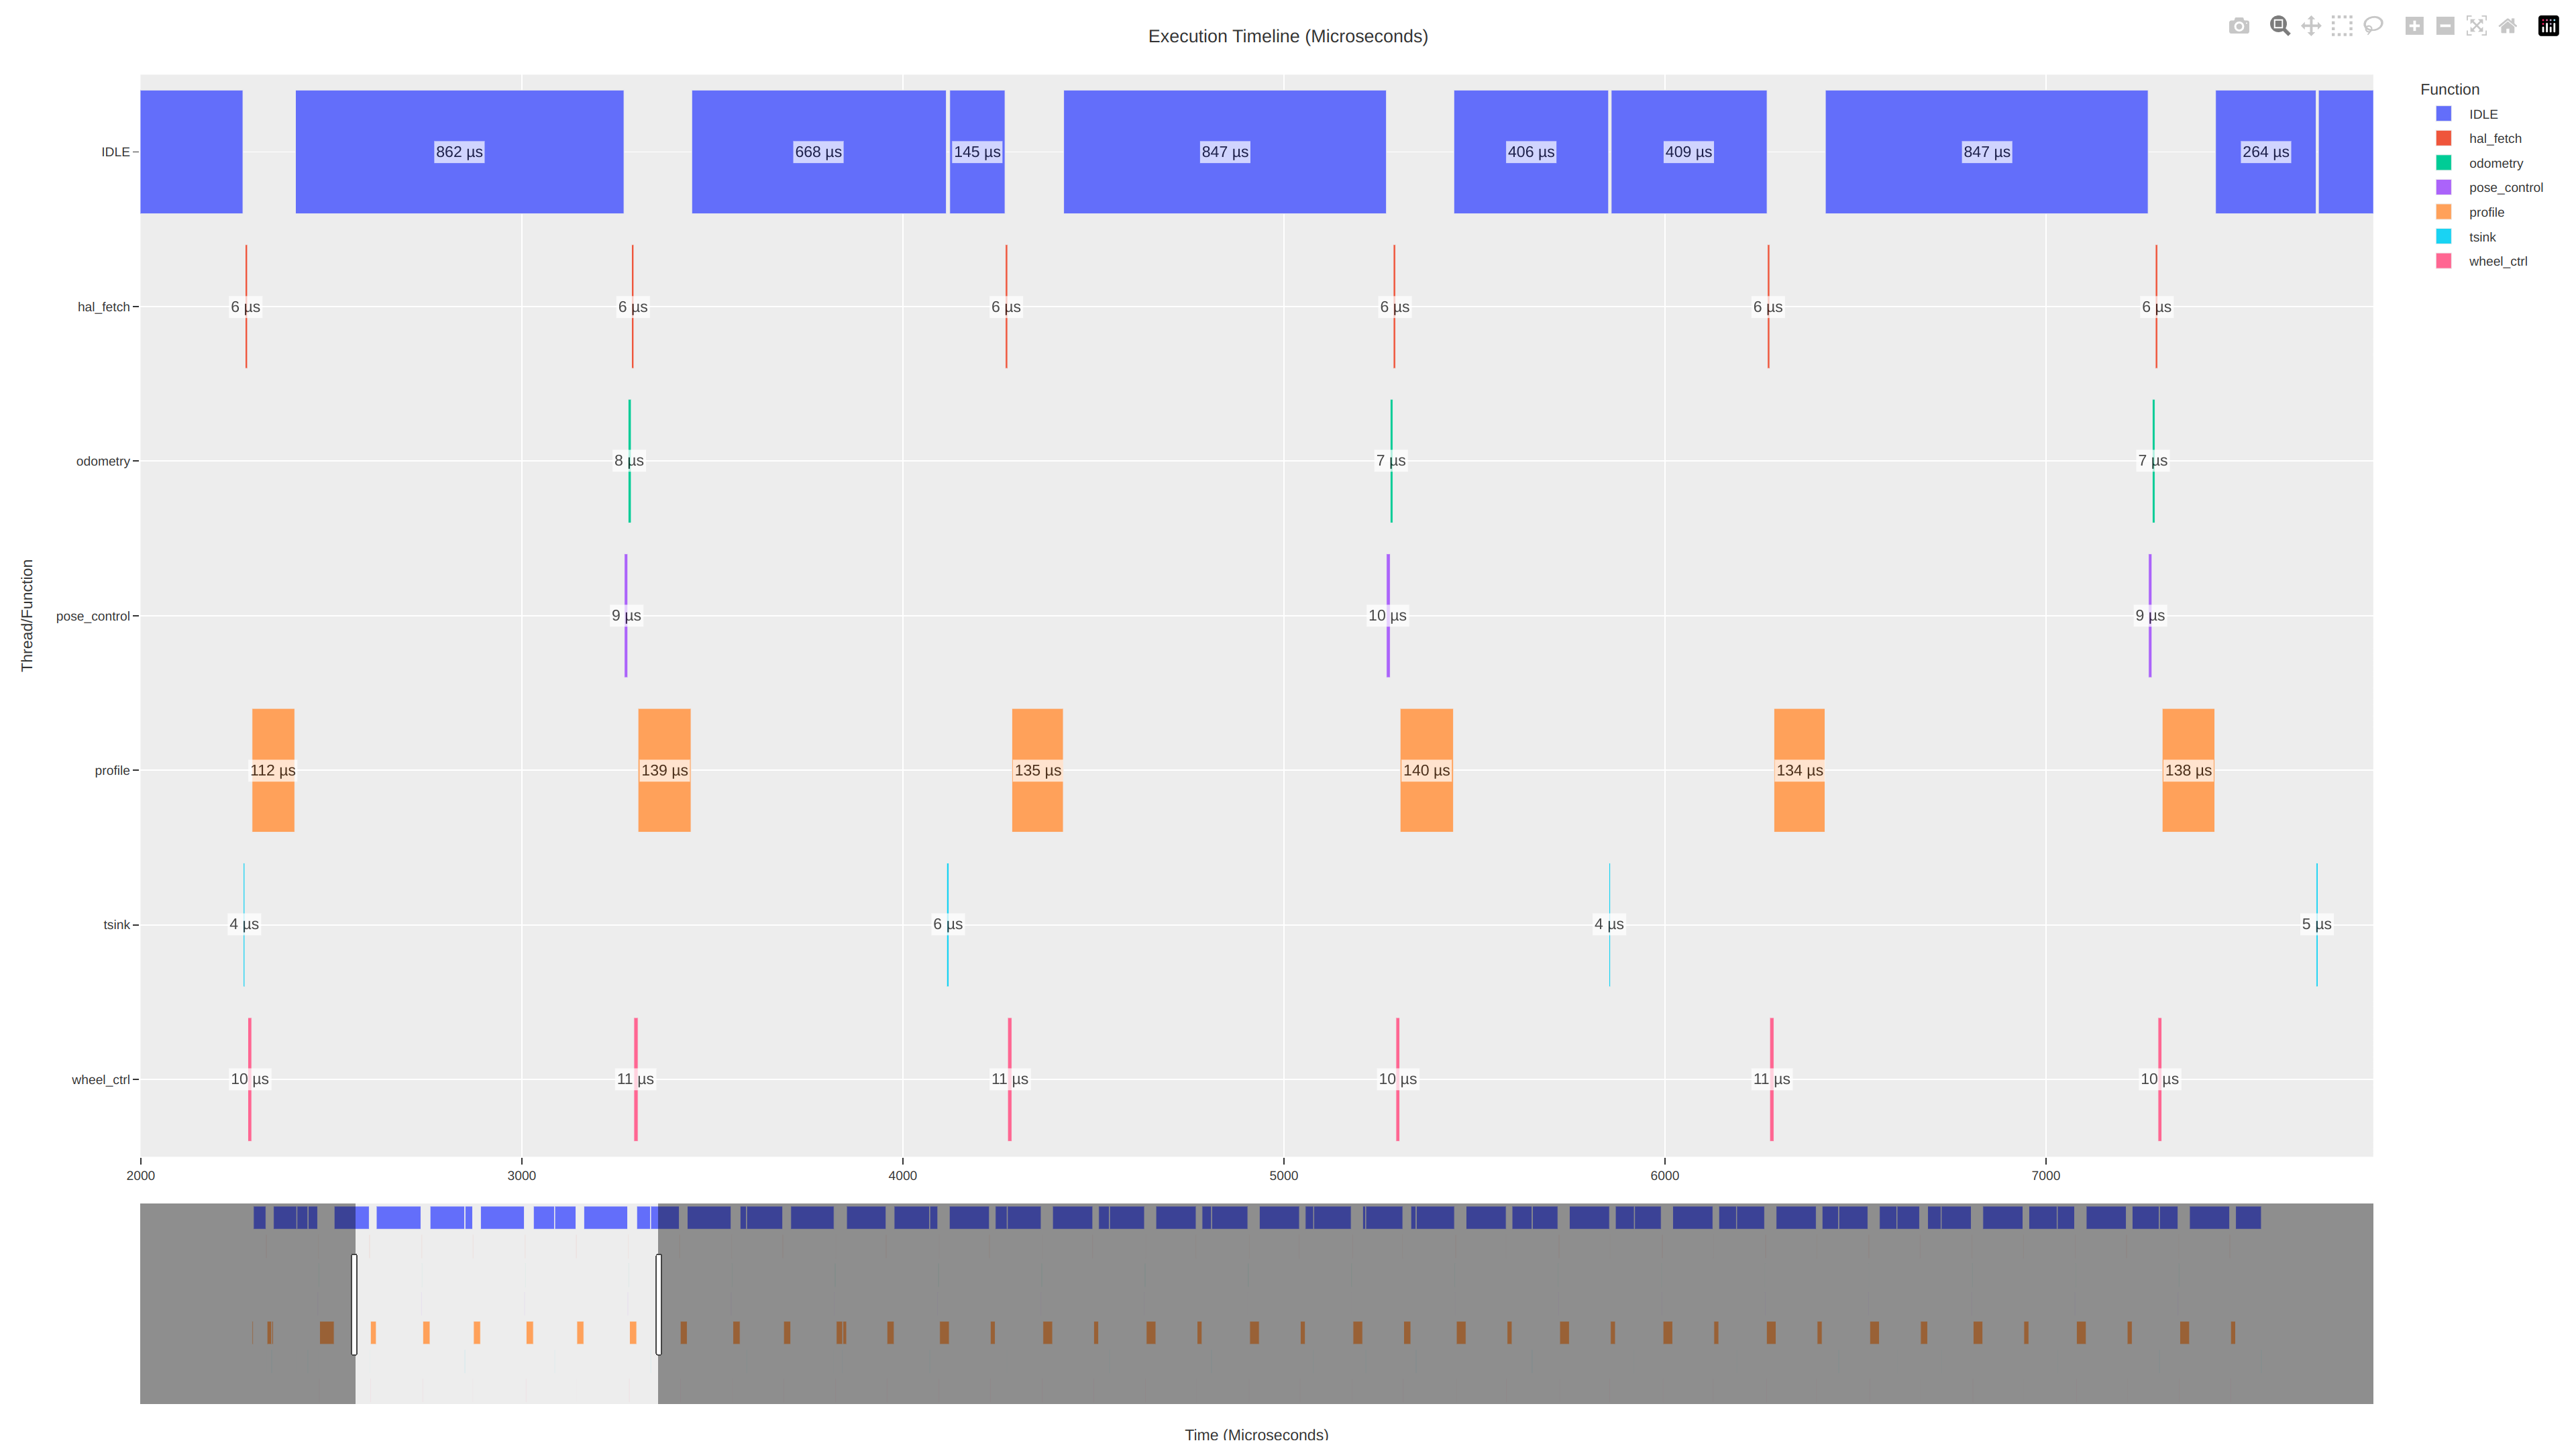
\includegraphics[width=1\textwidth]{assets/freertos_profiling_1000hz_ausschnitt}
    \caption{Laufzeit-Statistik mit 1000 Hz unter FreeRTOS -- Ausschnitt}
    \label{fig:freertos_1000hz_section}
\end{figure}

Bei einer $\textbf{5000\,\text{Hz}\text{|}2000\,\text{Hz}}$-Reglerkonfiguration
führt der Scheduler die Kontextwechsel weiterhin zuverlässig aus
(\ref{fig:freertos_5000hz}, \ref{fig:freertos_5000hz_section}). Die
Regelungsfunktionen werden in regelmäßigen Abständen von $200\,\mu\text{s}$ bzw.
$500\,\mu\text{s}$ aufgerufen (\ref{code:freertos_data_5000hz}). Das System
verbleibt bei diesen Frequenzen größtenteils ebenfalls im Leerlauf.

\begin{figure}[H]
    \centering
    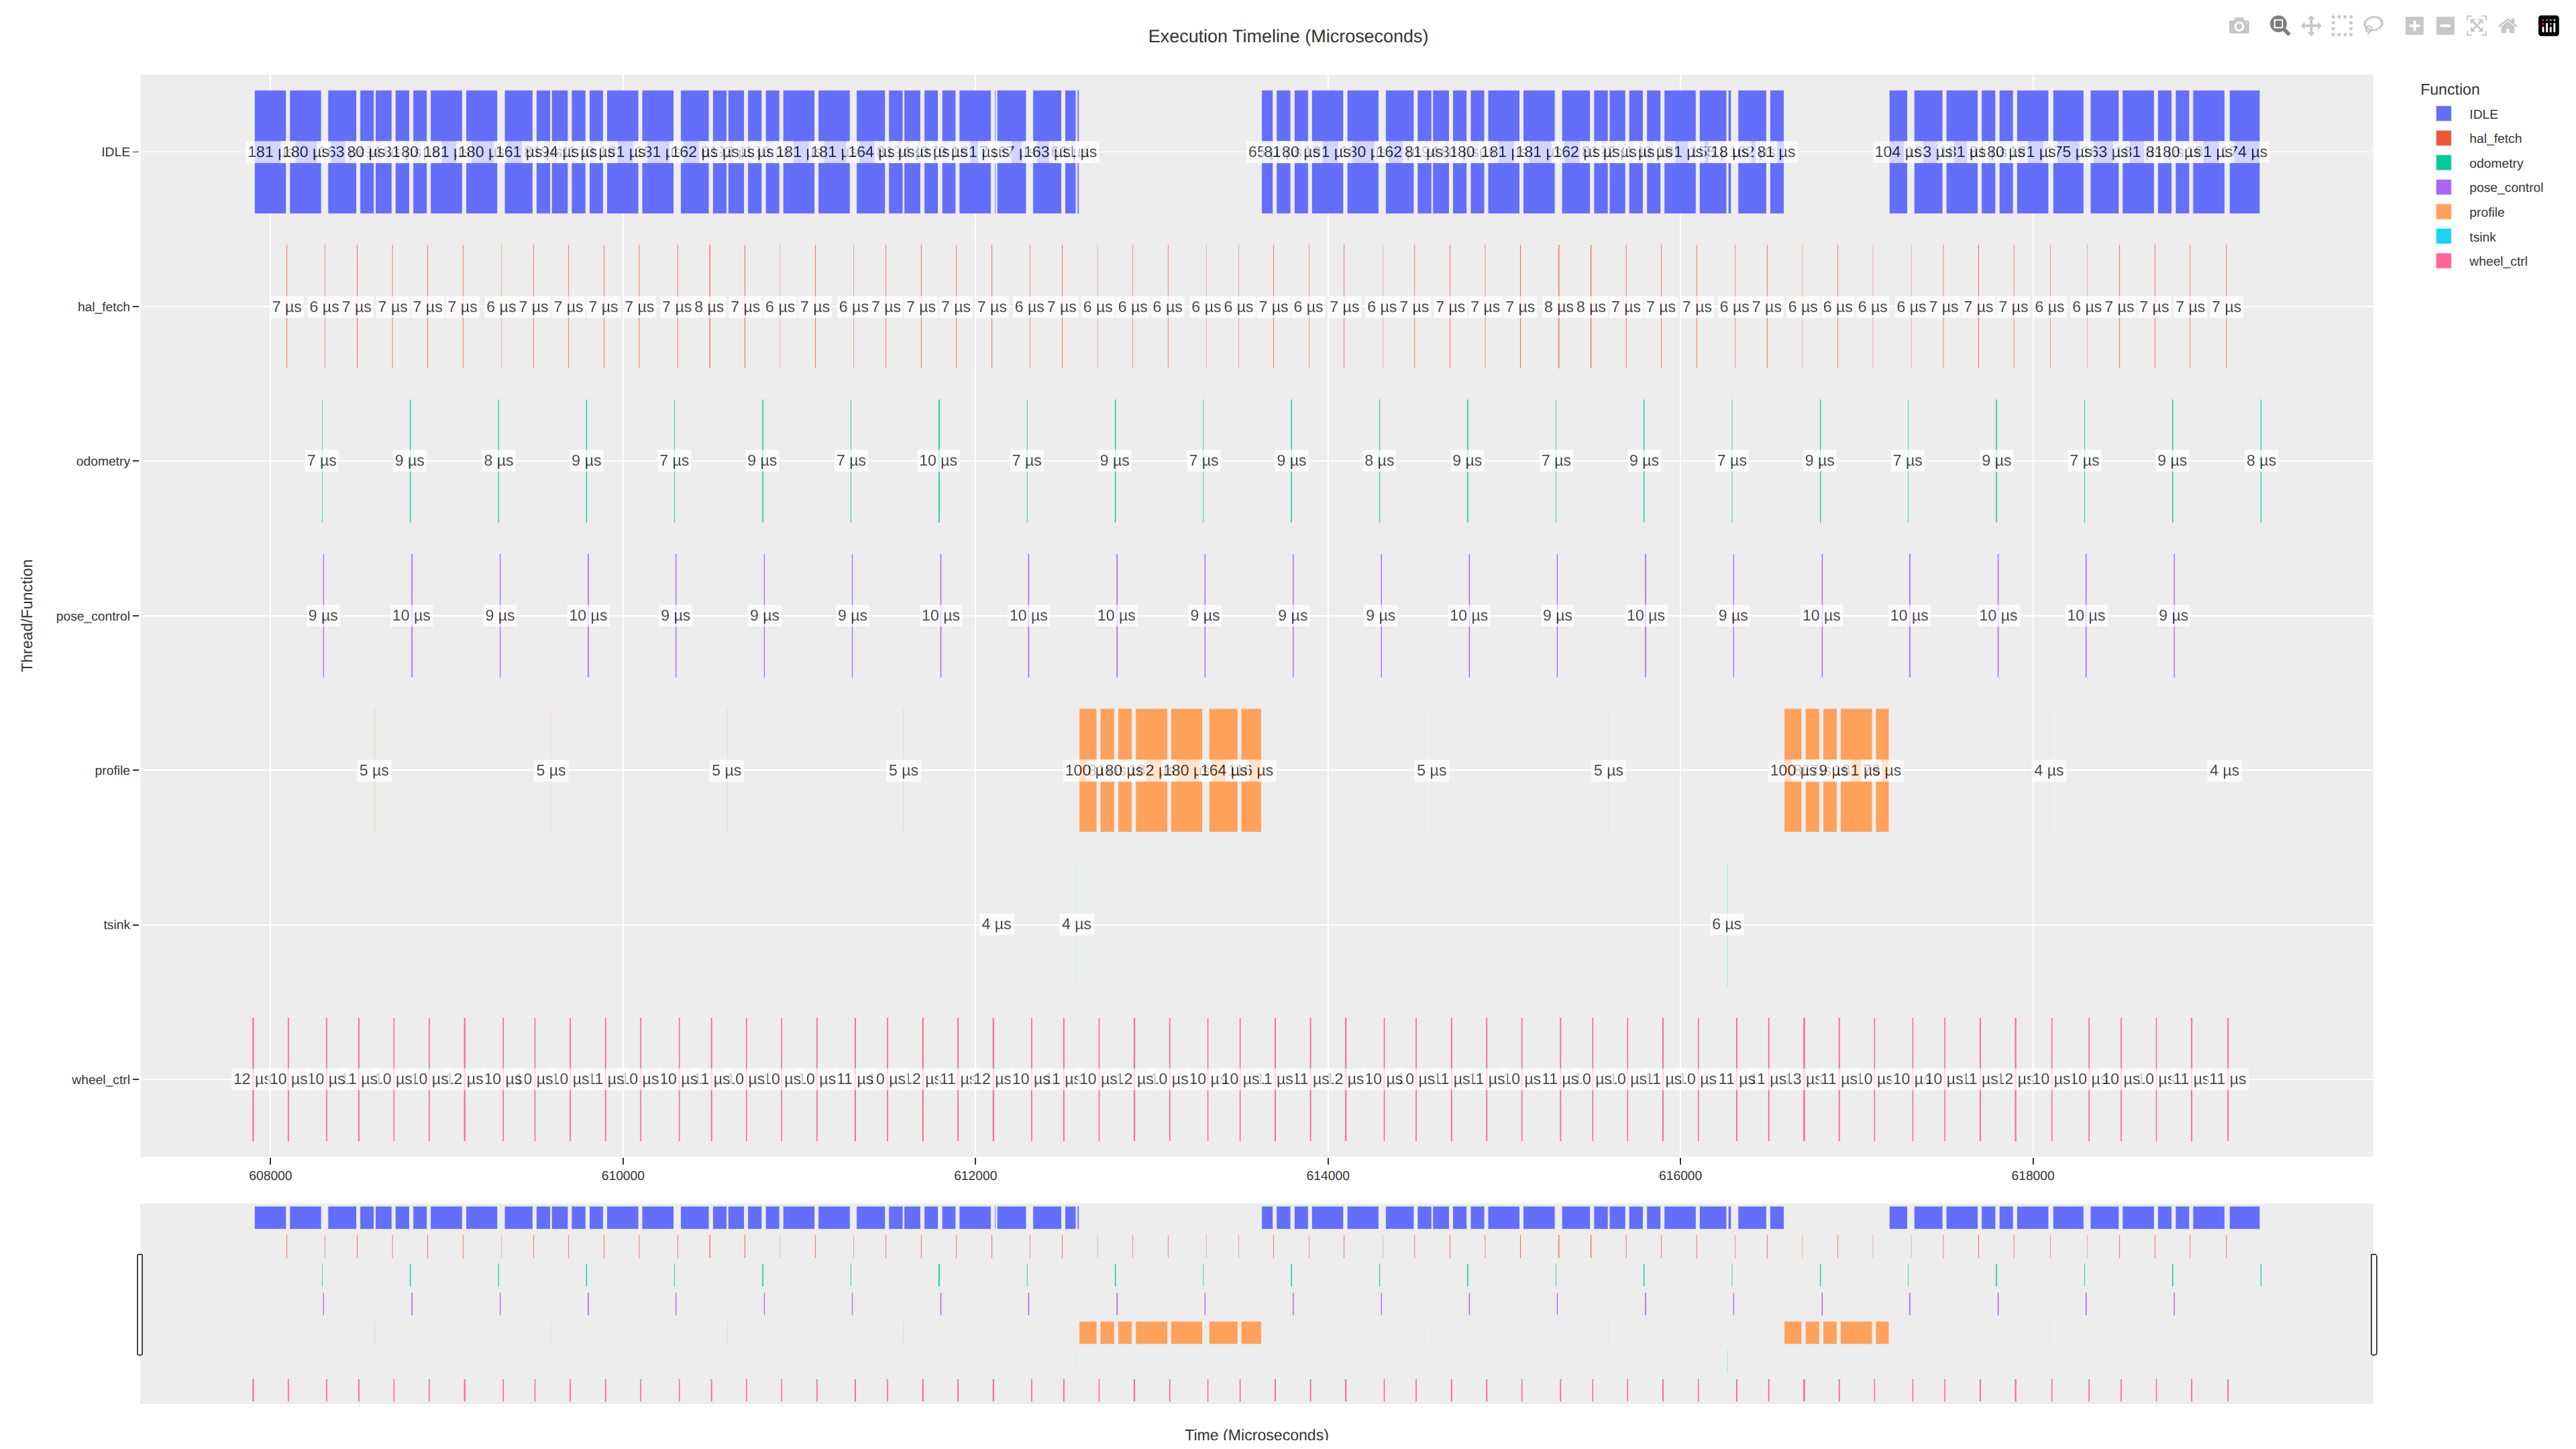
\includegraphics[width=1\textwidth]{assets/freertos_profiling_5000hz}
    \caption{Laufzeit-Statistik mit 5000 Hz unter FreeRTOS}
    \label{fig:freertos_5000hz}
\end{figure}
\begin{figure}[H]
    \centering
    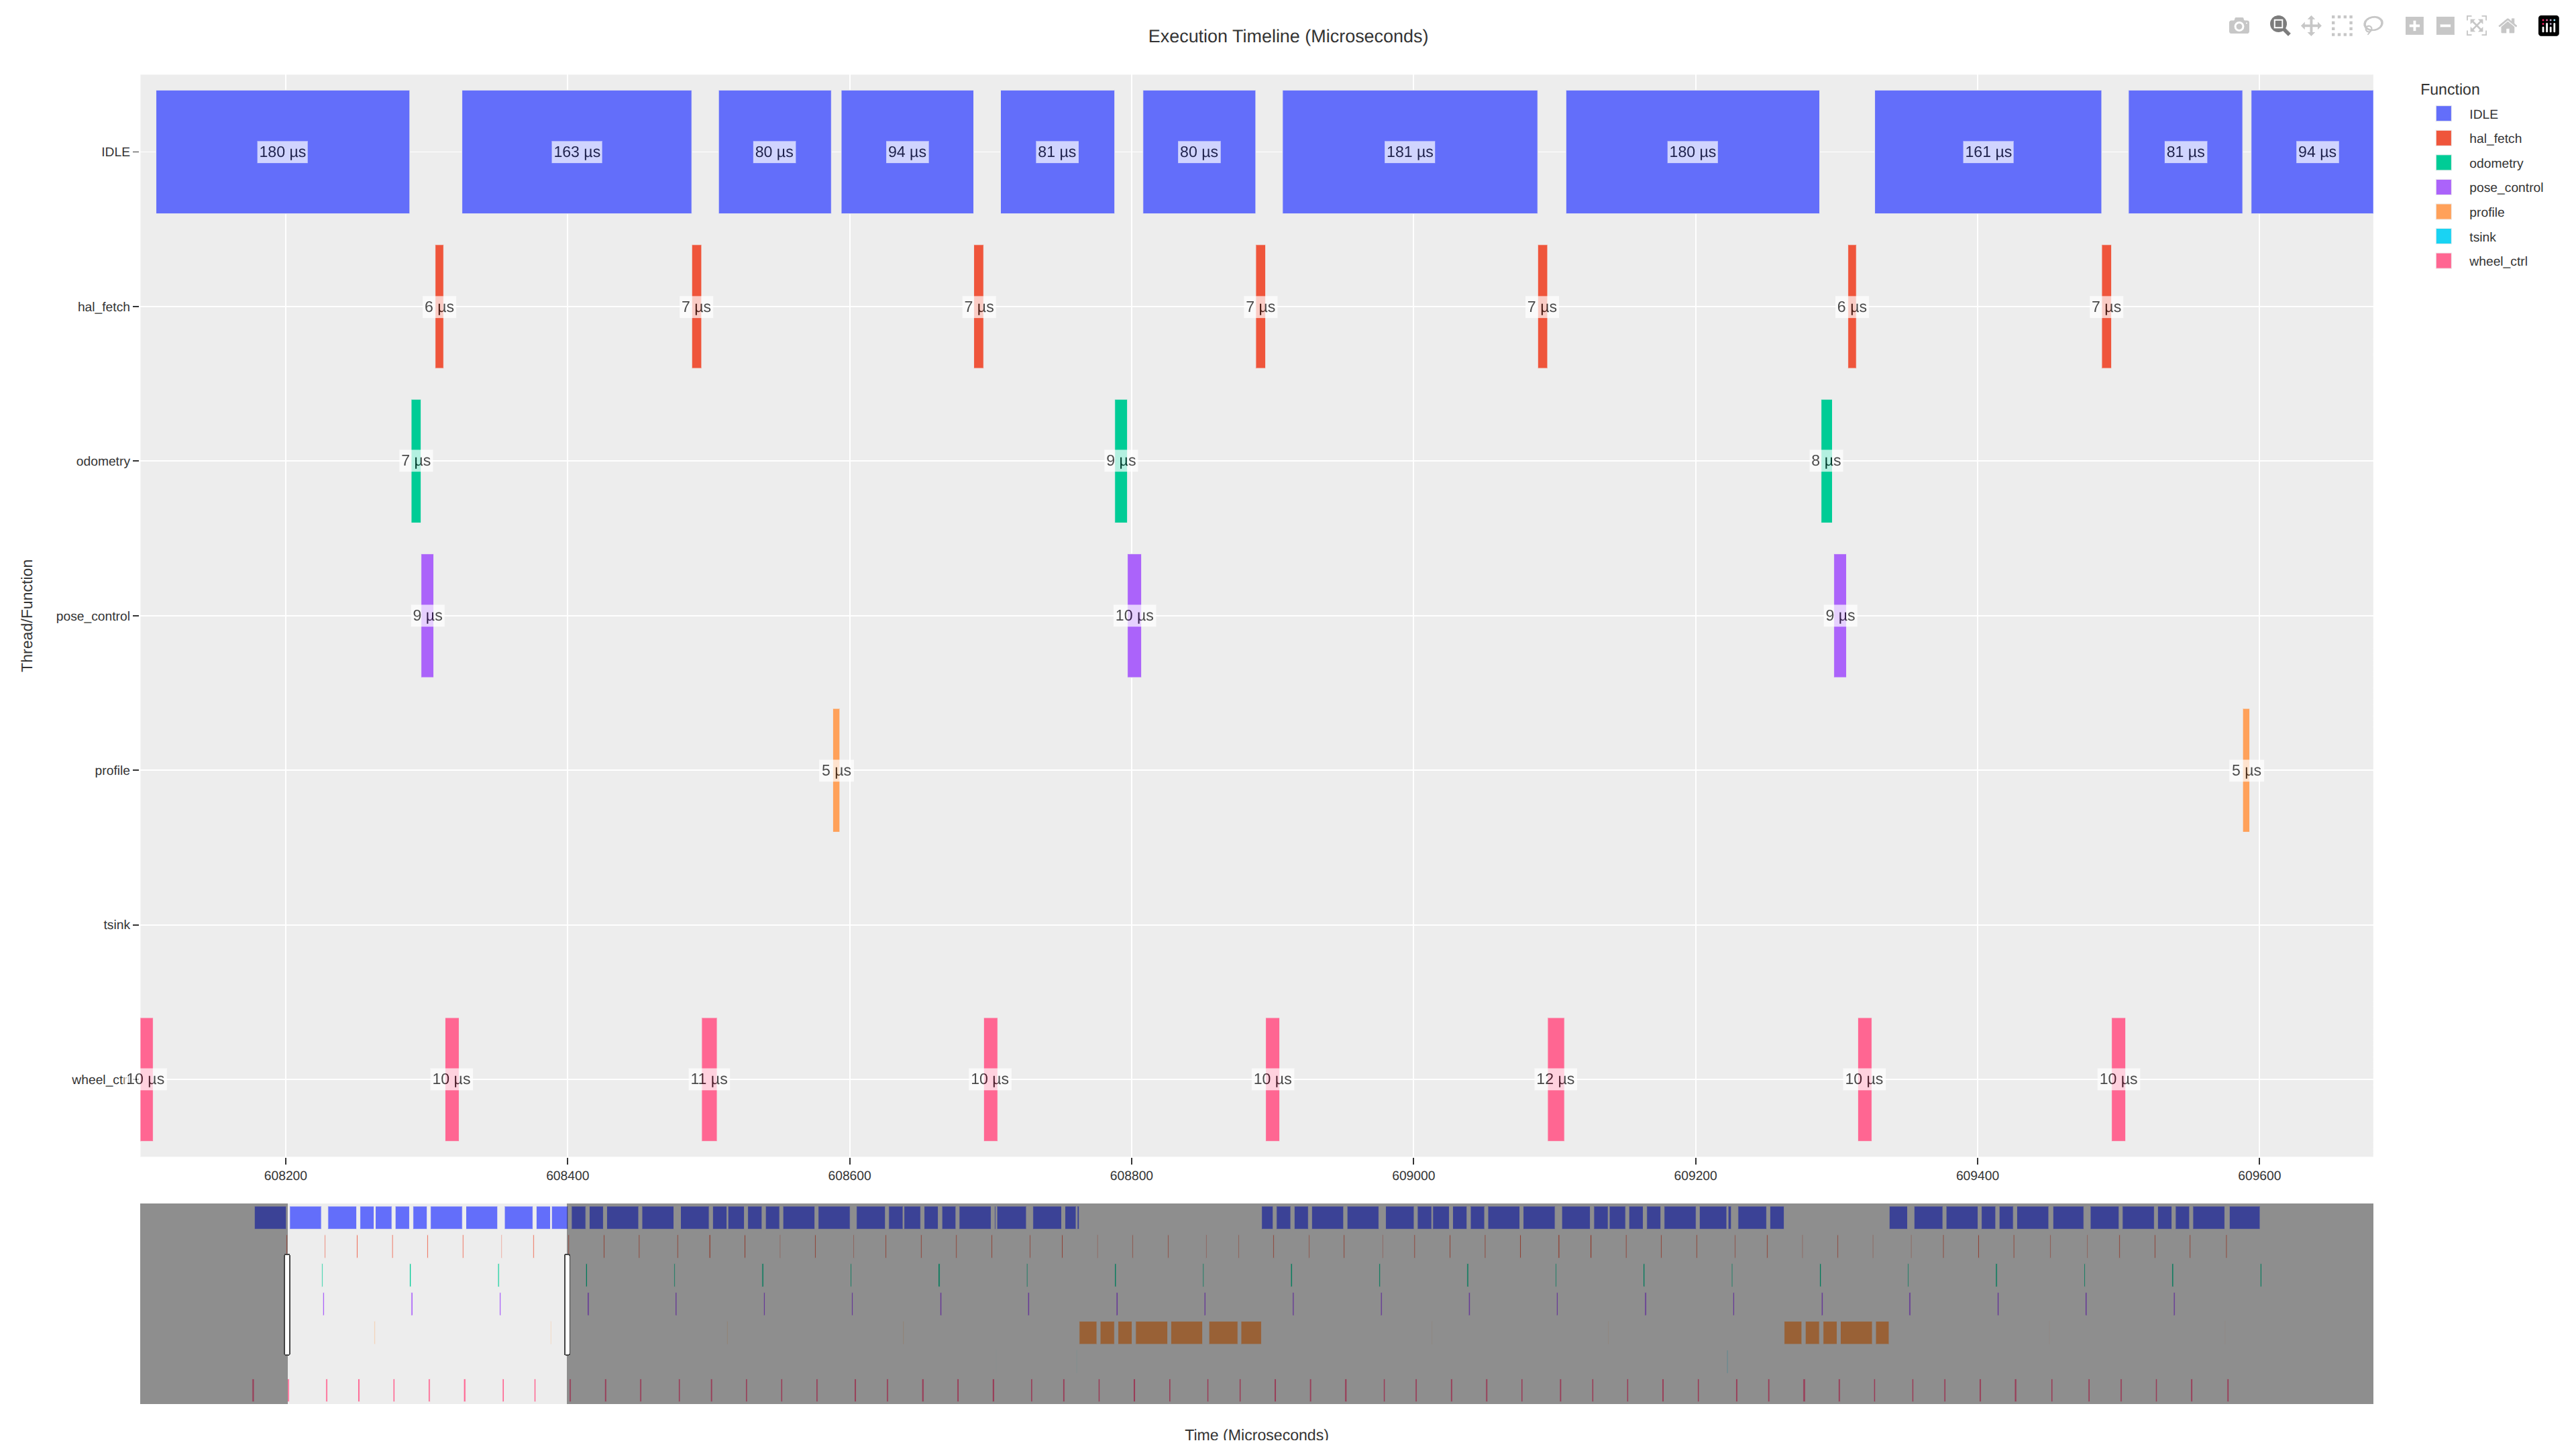
\includegraphics[width=1\textwidth]{assets/freertos_profiling_5000hz_ausschnitt}
    \caption{Laufzeit-Statistik mit 5000 Hz unter FreeRTOS -- Ausschnitt}
    \label{fig:freertos_5000hz_section}
\end{figure}

\begin{code}
\begin{minted}{cpp}
IDLE 1 0
profile 2 1
profile 25 0
IDLE 27 1
IDLE 88 0
hal_fetch 89 1
hal_fetch 95 0
wheel_ctrl 96 1     << Start einer Iteration (Drehzahl)
wheel_ctrl 106 0
IDLE 107 1
IDLE 288 0
odometry 289 1      << Start einer Iteration (Odometrie)
odometry 296 0
pose_control 297 1
pose_control 306 0
hal_fetch 307 1
hal_fetch 313 0
wheel_ctrl 313 1    << nach etwa 200 us zur vorherigen Iteration (Drehzahl)
...
odometry 788 1      << nach etwa 500 us zur vorherigen Iteration (Odom)
\end{minted}
    \captionof{listing}{Profiling-Daten bei 5000|2000Hz}
    \label{code:freertos_data_5000hz}
\end{code}

Selbst bei einer $\textbf{10000\,\text{Hz}|5000\,\text{Hz}}$-Konfiguration zeigt
das System ein relativ zuverlässiges Laufzeitverhalten ohne vollständige
Prozessorauslastung (\ref{fig:freertos_10000hz},
\ref{fig:freertos_10000hz_section}, \ref{code:freertos_data_10000hz}) --
abgesehen von der Profiling-Task. Hier wird vermutlich die zugrundeliegende
Übertragung zum Bottleneck: Die hohen Takt- und Regelungsfrequenzen erzeugen
Datenmengen, die nicht mehr rechtzeitig vom DMA-Controller verarbeitet werden
können, was zu periodischen Pufferüberläufen führt.

\begin{figure}[H]
    \centering
    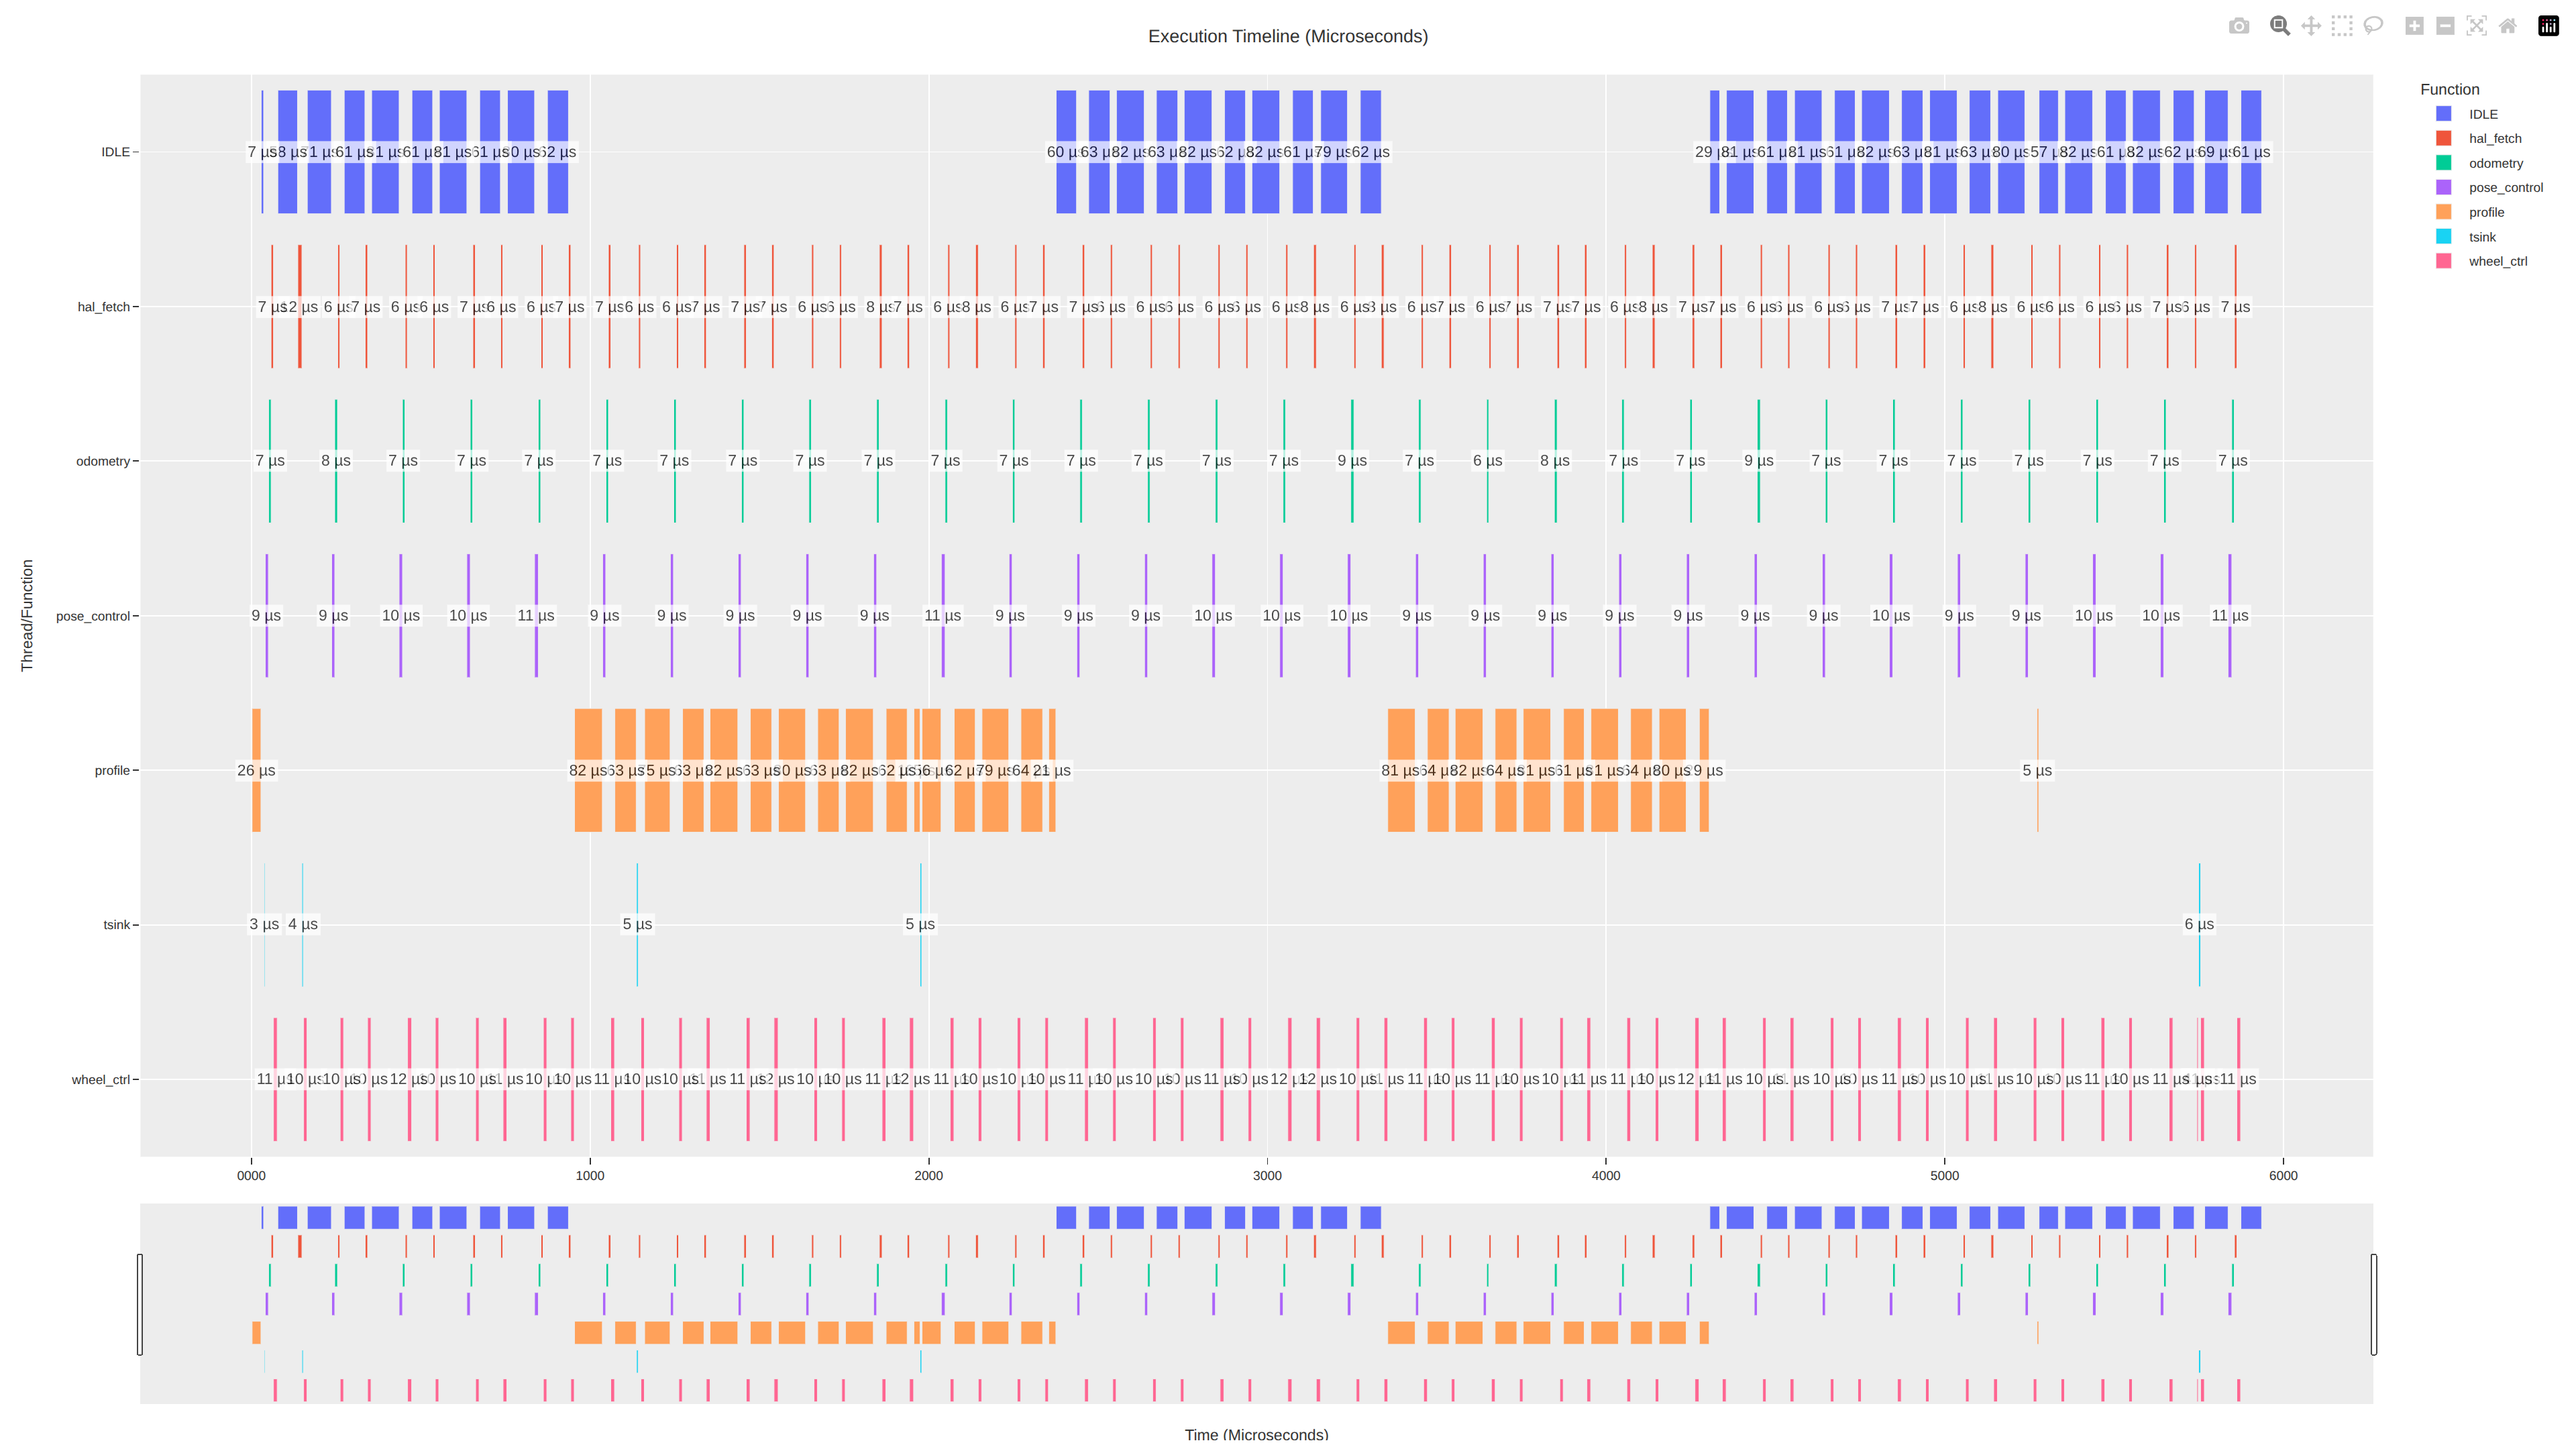
\includegraphics[width=1\textwidth]{assets/freertos_profiling_10000hz}
    \caption{Laufzeit-Statistik mit 10000 Hz unter FreeRTOS}
    \label{fig:freertos_10000hz}
\end{figure}
\begin{figure}[H]
    \centering
    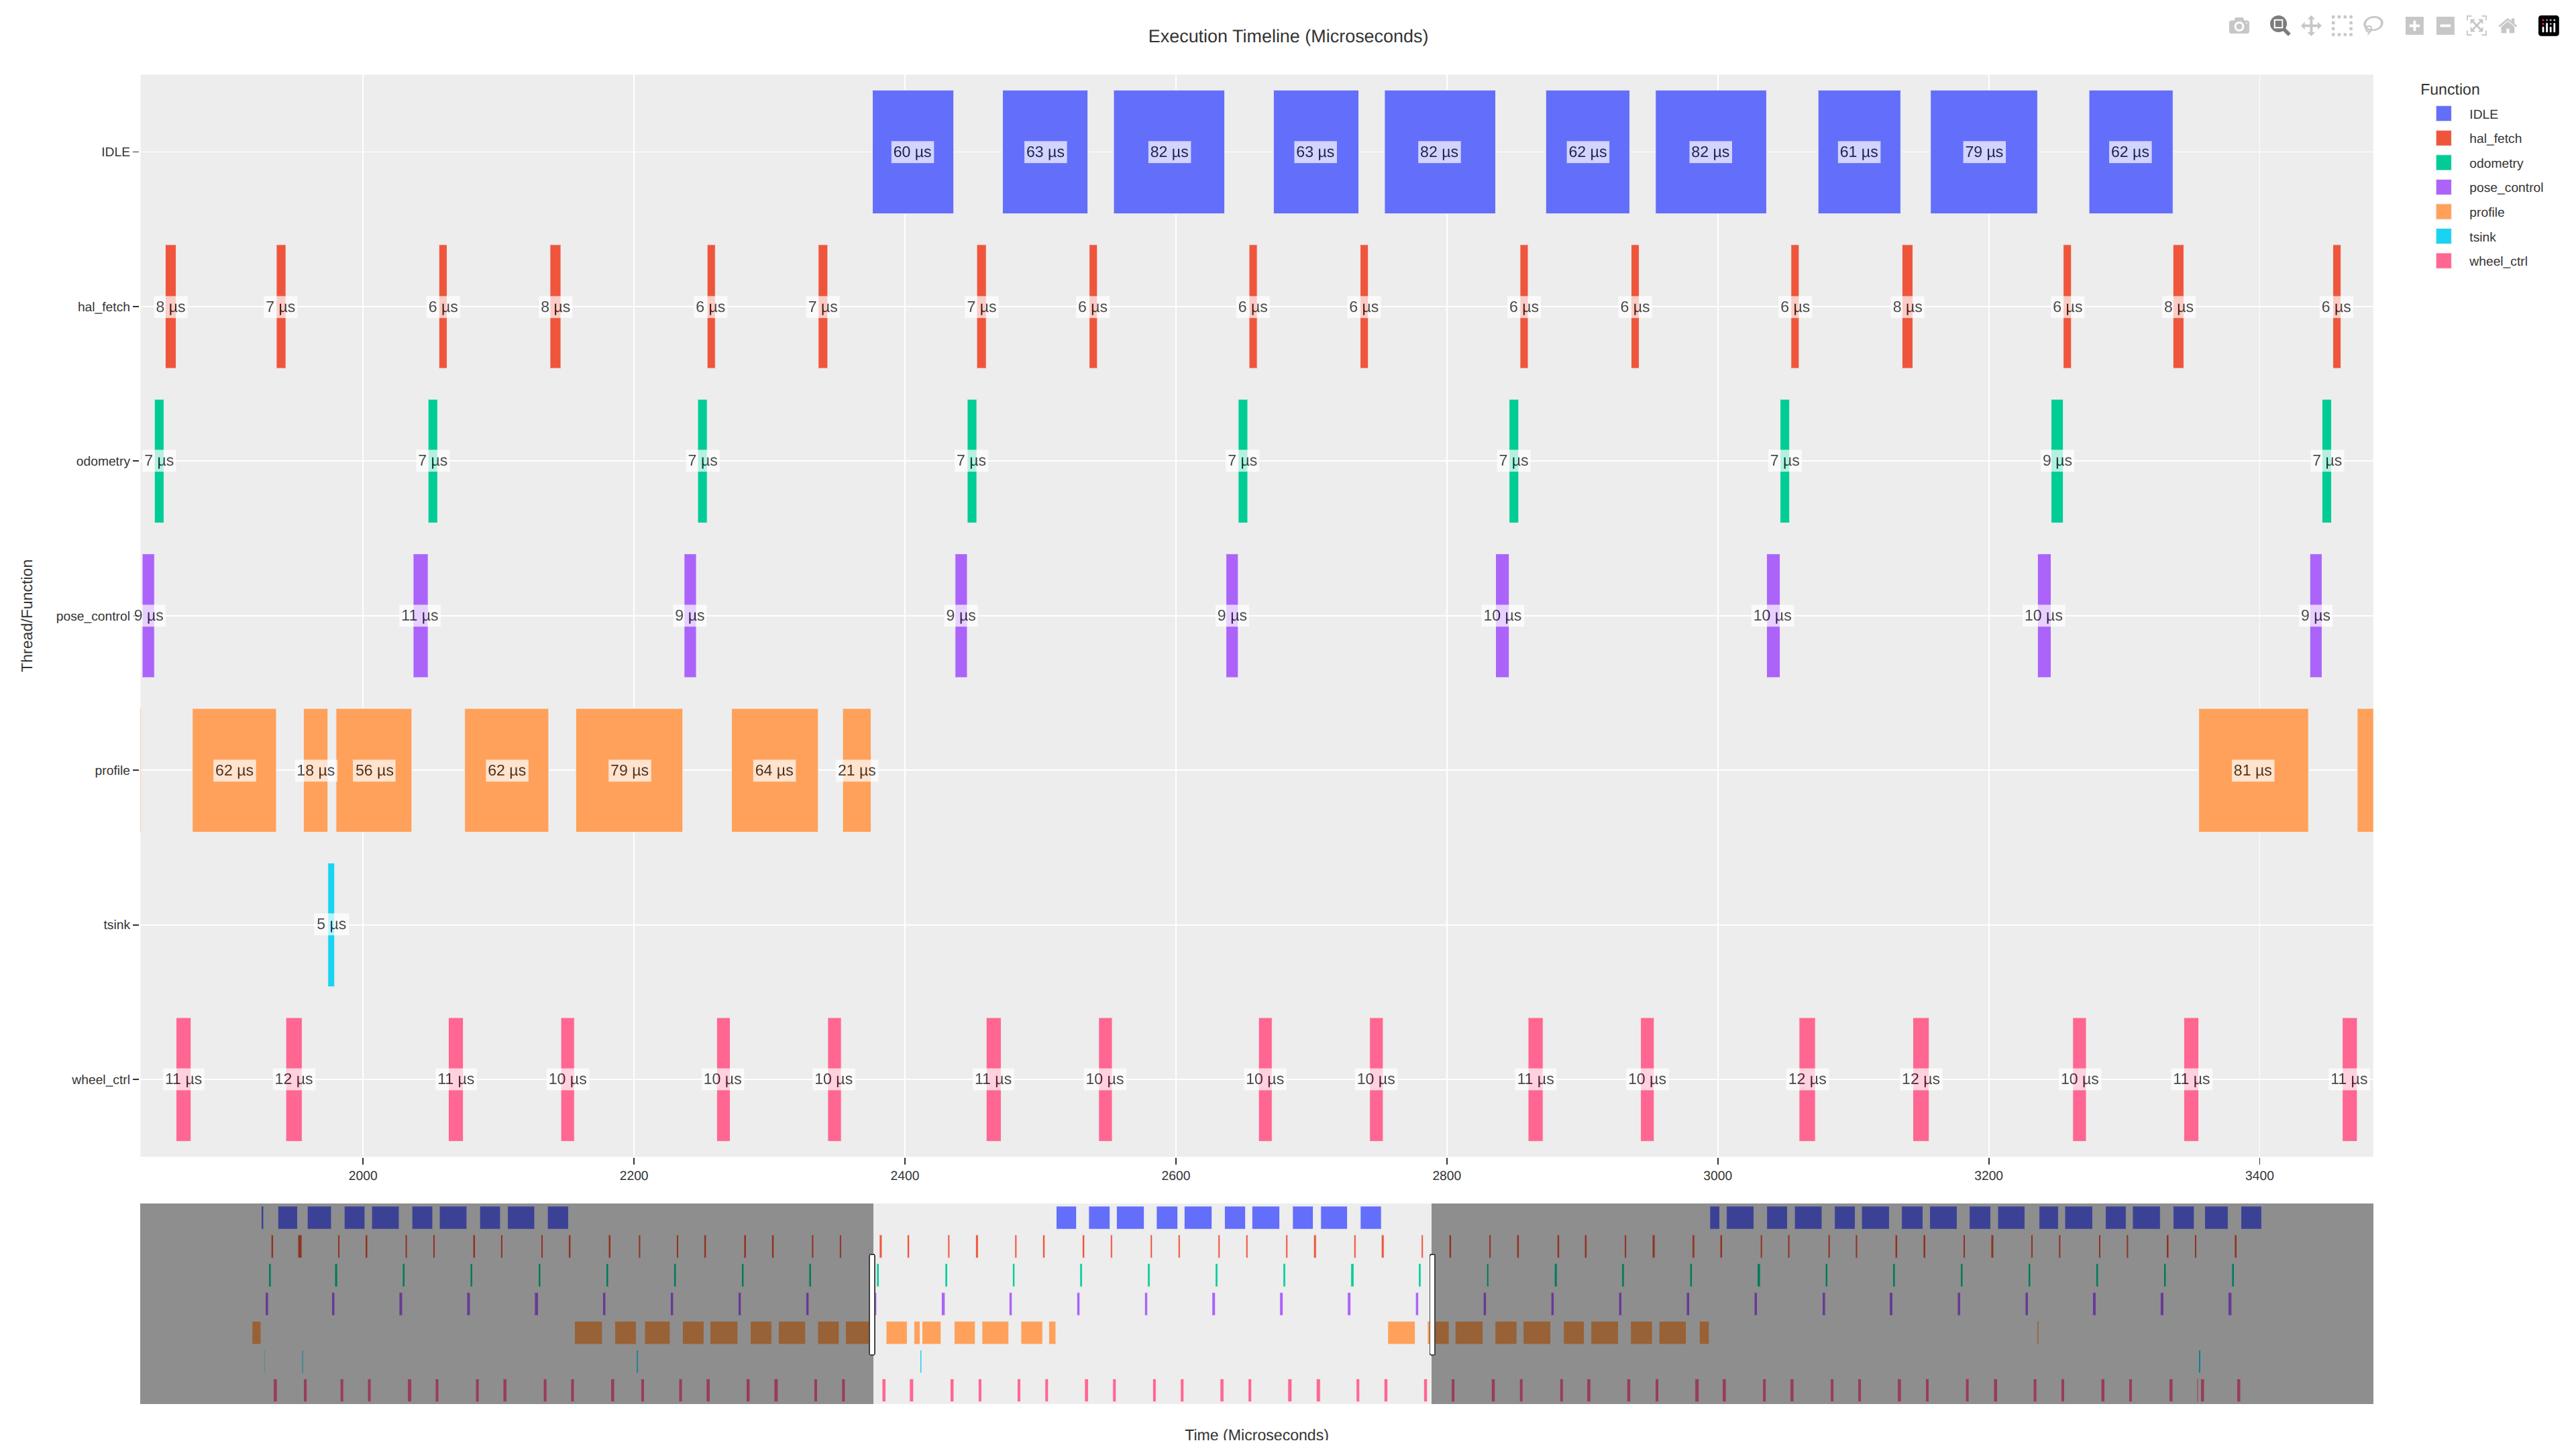
\includegraphics[width=1\textwidth]{assets/freertos_profiling_10000hz_ausschnitt}
    \caption{Laufzeit-Statistik mit 10000 Hz unter FreeRTOS -- Ausschnitt}
    \label{fig:freertos_10000hz_section}
\end{figure}

\begin{code}
\begin{minted}{cpp}
profile 2 1
profile 28 0
IDLE 29 1
IDLE 36 0
tsink 37 1
tsink 40 0
pose_control 41 1   << Start einer Iteration (Pose)
pose_control 50 0
odometry 51 1
odometry 58 0
hal_fetch 58 1
hal_fetch 65 0
wheel_ctrl 65 1     << Start einer Iteration (Drehzahl)
wheel_ctrl 76 0
IDLE 78 1
IDLE 136 0
hal_fetch 137 1
hal_fetch 149 0
tsink 149 1
tsink 153 0
wheel_ctrl 154 1    << nach etwa 100 us zur vorherigen Iteration (Drehzahl)
wheel_ctrl 164 0
IDLE 165 1
IDLE 236 0
pose_control 237 1  << nach etwa 200 us zur vorherigen Iteration (Pose)
pose_control 246 0
...
\end{minted}
    \captionof{listing}{Profiling-Daten bei 10000|5000Hz}
    \label{code:freertos_data_10000hz}
\end{code}

Micro-ROS erreichte eine Sollfrequenz von $1000\,\text{Hz}$ nicht und wies
stattdessen Schwankungen zwischen $910\,\text{Hz}$ und $980\,\text{Hz}$ auf
(\ref{fig:uros_1000hz}, \ref{fig:uros_1000hz_section}). Dies lässt sich
vermutlich auf zwei Hauptfaktoren zurückführen: Erstens wird die maximal
erreichbare Frequenz durch die Integration der zusätzlichen Middleware
beeinflusst \cite{ROS_Performance2019} -- konkret \ac{XRCE}-DDS seitens
Micro-ROS und standardmäßig Fast DDS bei ROS2.

Zweitens könnte der inhärente Overhead des ROS/Micro-ROS-Stacks ebenfalls
signifikante Latenzen verursachen, da alle Daten zwingend als gepackte Pakete
über eine UDP-basierte Verbindung zum Linux-Host und zurück übertragen werden
müssen. Dieser transportbedingte, plattformübergreifende Mechanismus führt zu
zusätzlichen nicht-deterministischen Verzögerungen im Gegensatz zur
FreeRTOS-Implementierung, bei der der Datenaustausch vollständig intern durch
direkte Speicherkopien zwischen Adressräumen realisiert wird.

\begin{figure}[H]
    \centering
    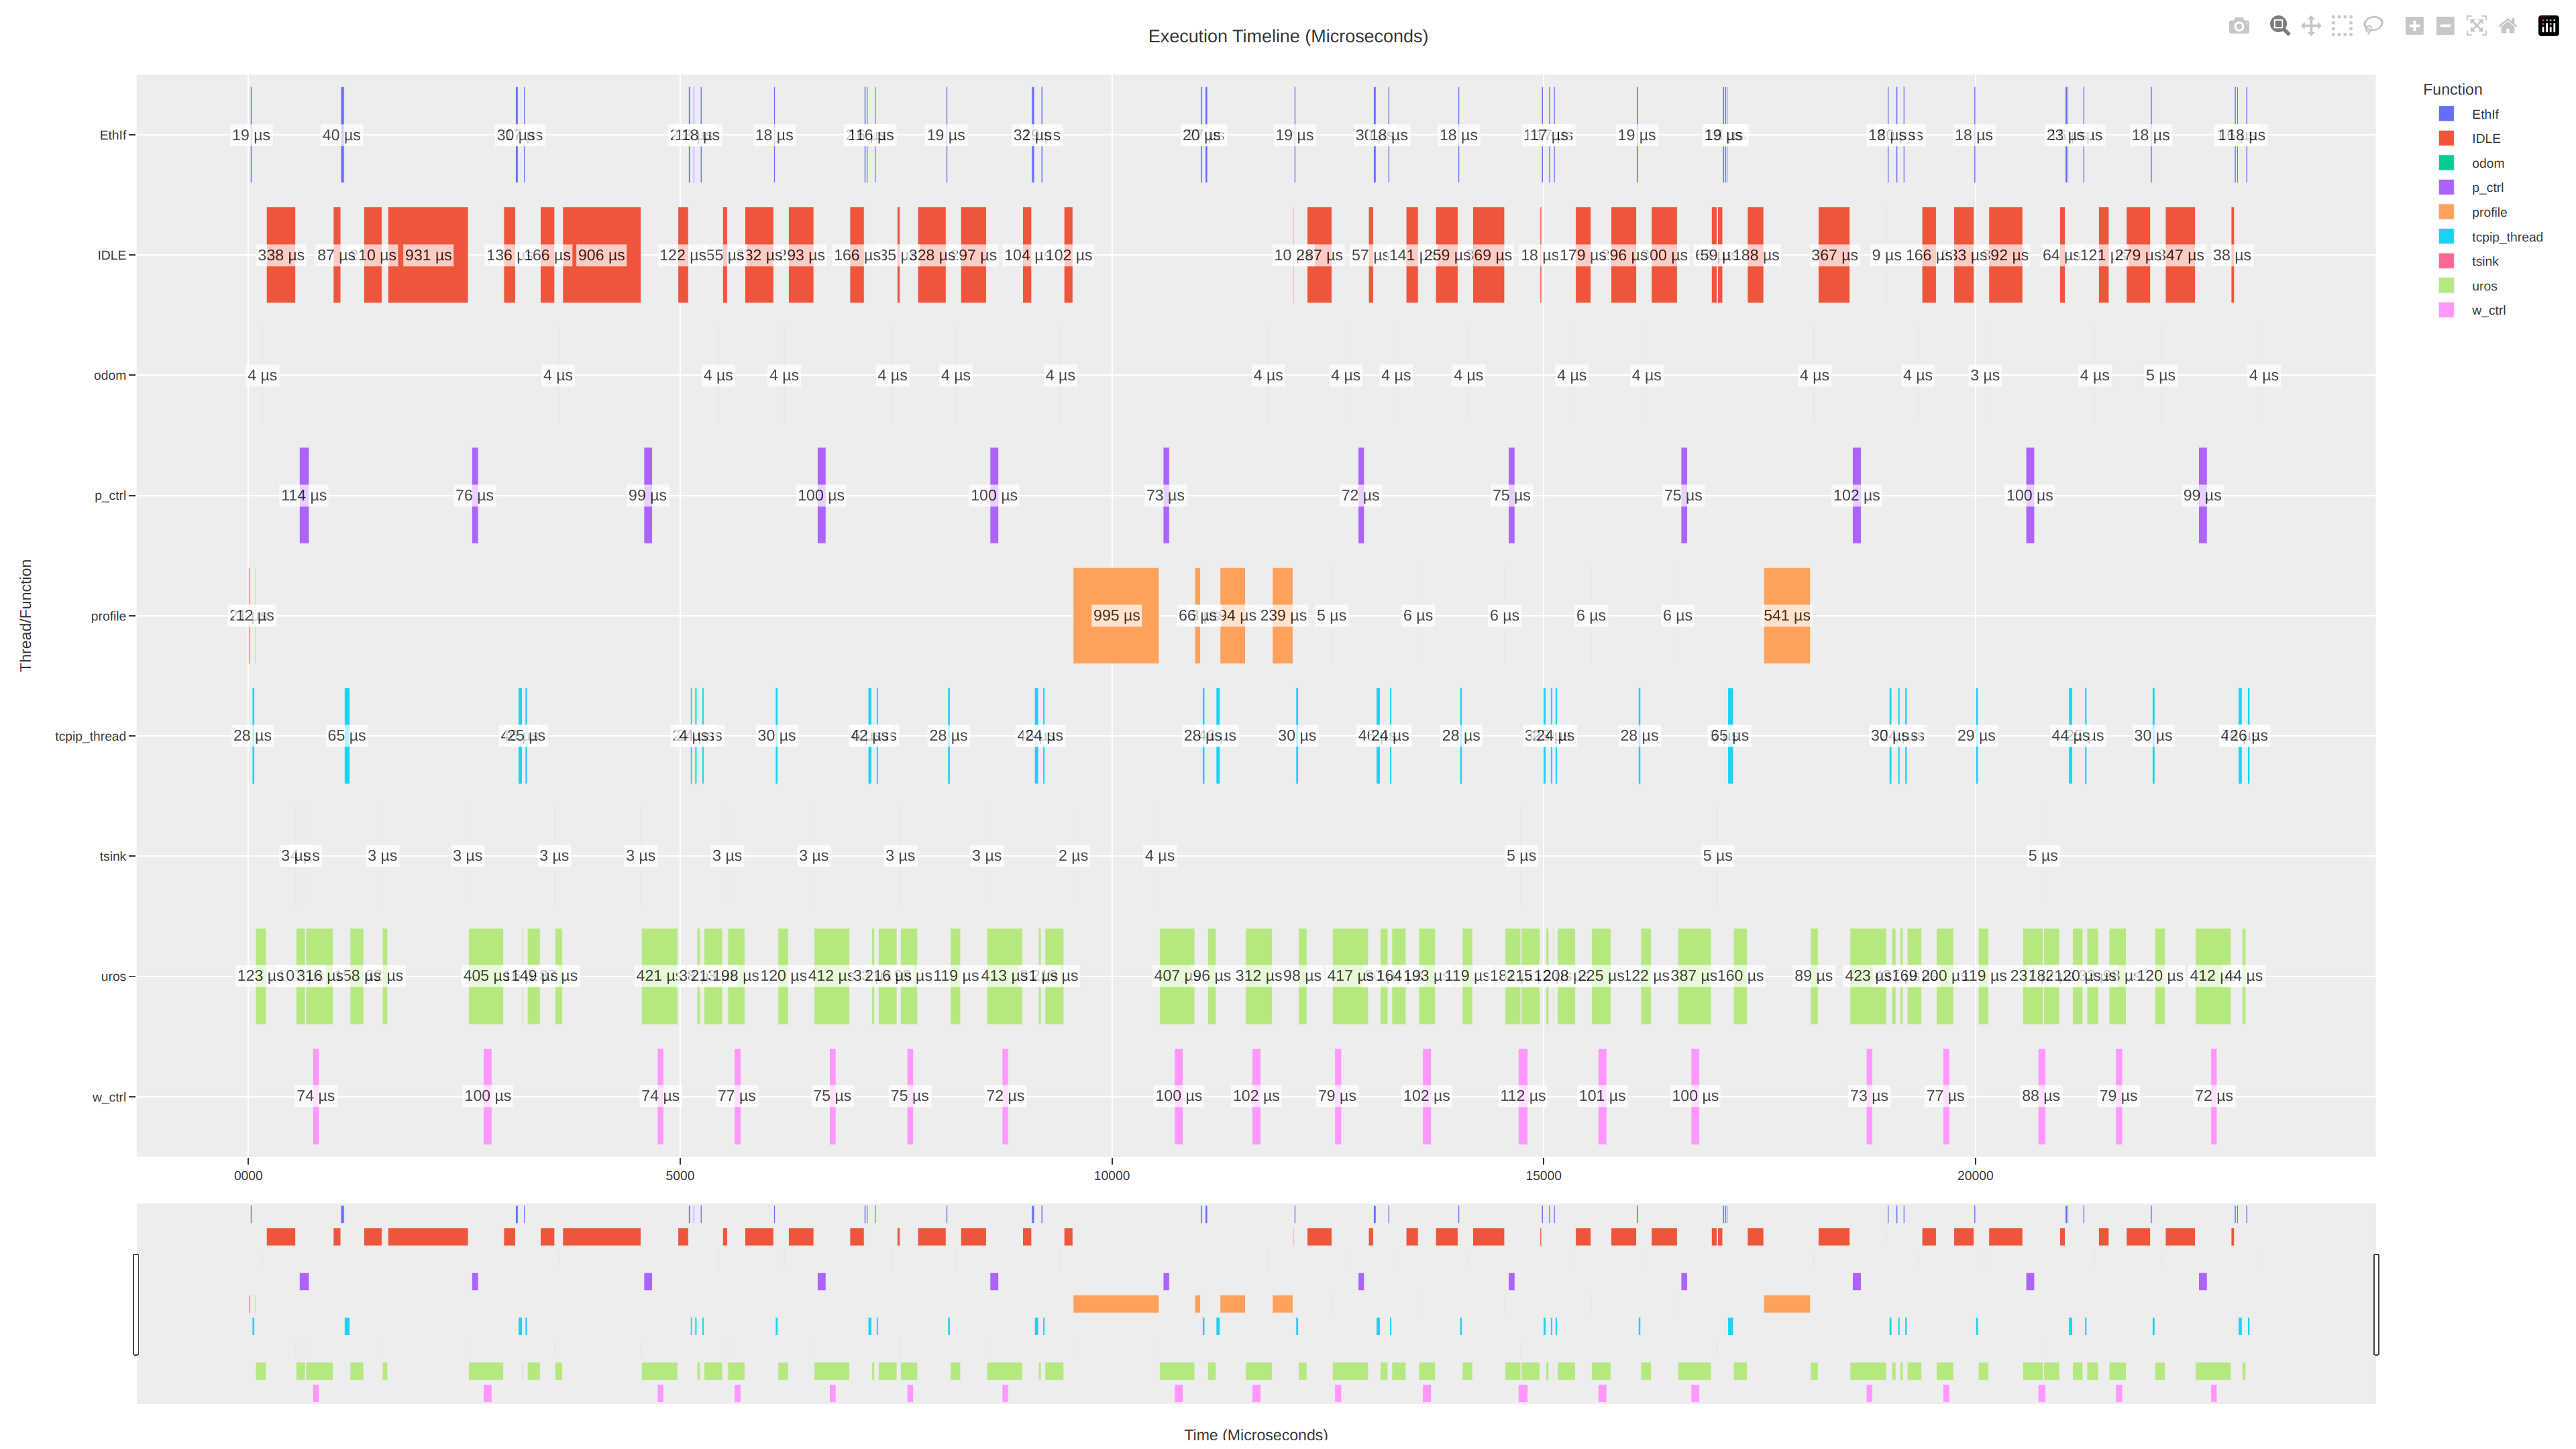
\includegraphics[width=1\textwidth]{assets/micro_ros_profiling_1000hz}
    \caption{Laufzeit-Statistik mit 1000 Hz unter Micro-ROS}
    \label{fig:uros_1000hz}
\end{figure}
\begin{figure}[H]
    \centering
    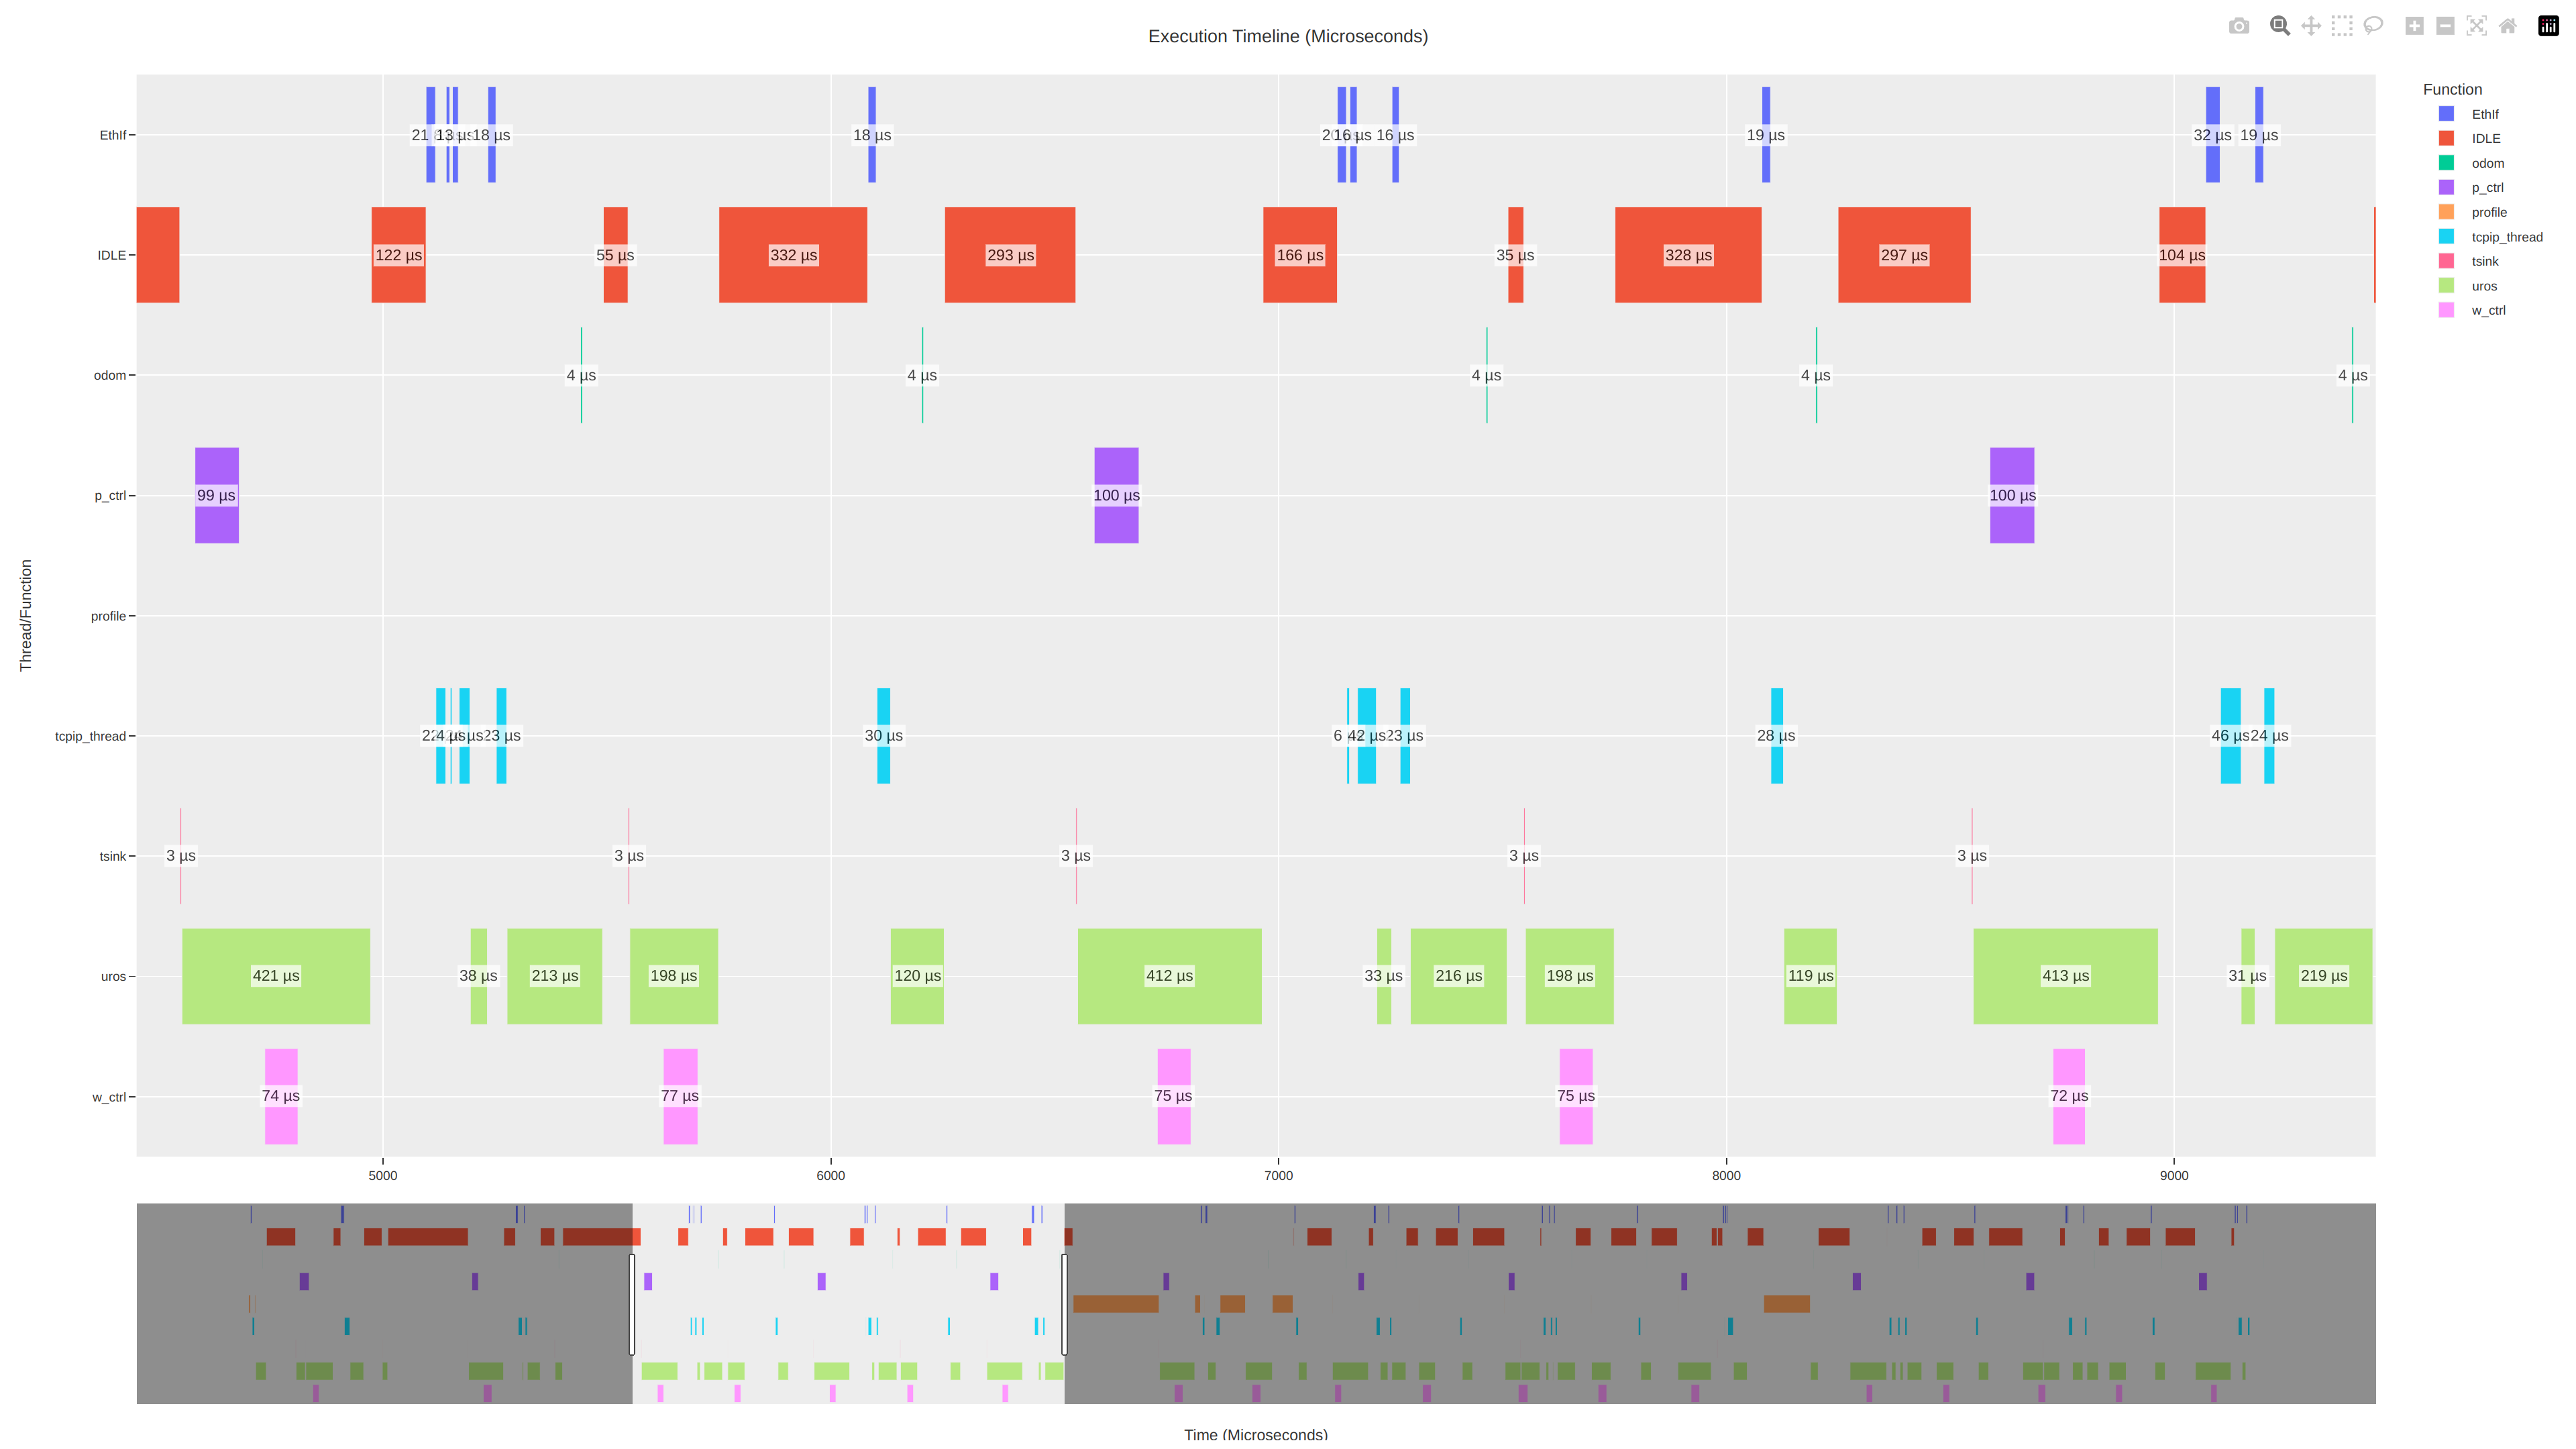
\includegraphics[width=1\textwidth]{assets/micro_ros_profiling_1000hz_ausschnitt}
    \caption{Laufzeit-Statistik mit 1000 Hz unter Micro-ROS -- Ausschnitt}
    \label{fig:uros_1000hz_section}
\end{figure}

\subsubsection{Dauer von Regelungsfunktionen}

Aus den Profiling-Daten lässt sich ebenfalls folgender Vergleich
(\ref{table:comparison_control_fn}) zwischen den beiden Implementierungen
ableiten:

\begin{table}[h]
\centering
\begin{tabular}{|l|r|r|r|}
\hline
    \textbf{Name} & \textbf{Micro-ROS (\text{µs})} & \textbf{FreeRTOS (\text{µs})} & \textbf{Differenz (\text{µs})} \\ \hline
    Odometrie & 6.780 (Ø:~3,74) & 6.256 (Ø:~6,84) & -524 (Ø: -3,10) \\ \hline
Posenregelung & 69.301 (Ø:~75,16) & 9.043 (Ø:~9,88) & 60.258 (Ø:~65,28) \\ \hline
Drehzahlregelung & 191.027 (Ø:~103,59) & 19.559 (Ø:~10,69) & 171.468 (Ø:~92,90) \\ \hline
\end{tabular}
\caption{Vergleich der Rechenzeiten zwischen Micro-ROS und FreeRTOS}
    \label{table:comparison_control_fn}
\end{table}

Die Implementierung ist auf beiden Plattformen größtenteils identisch, abgesehen
vom erwähnten Datenaustausch. Bei Micro-ROS müssen alle zu übertragenden Daten
in eine dedizierte Struktur mit Metadaten -- unter anderem einem Header mit
Zeitstempel in Sekunden und Nanosekunden -- serialisiert werden. Bei FreeRTOS
werden die Daten als rohe Bytes direkt in die Queue kopiert und beim Empfänger
extrahiert.

Zusätzlich unterscheidet sich die FreeRTOS-Implementierung von Micro-ROS auch
dadurch, dass die Encoderdaten nicht vom Drehzahlregler abgefragt und dann erst
an die Odometrie übergeben werden. Stattdessen übernimmt eine dedizierte
FreeRTOS-Task (\ref{code:enc_data_task}) die Übertragung dieser Daten sowohl an
den Drehzahlregler als auch an die Odometrie. Dadurch wird ein Teil des
Overheads vom Drehzahlregler entkoppelt.

Zusammenfassend zeigt sich, dass die Steuerungslogik sowohl unter Micro-ROS als
auch unter FreeRTOS relativ wenig Rechenzeit beansprucht -- vorausgesetzt, dass
die Daten ordentlich gecacht sind und nicht bei jedem Zugriff neu aus dem RAM
oder Flash geladen werden müssen. Unter FreeRTOS kann selbst bei deutlich
höheren Taktfrequenzen ein stabiler Kontextwechsel gewährleistet werden. Dank
des leistungsstarken Mikrocontrollers in Kombination mit Cache-Nutzung und
hardware- sowie softwareseitig optimiertem Code befindet sich das System auf
beiden Plattformen ebenfalls überwiegend im Leerlauf.
